In this section, we conduct a comprehensive comparison of the performance of POGPN with various models, including independent GPs (IGP), Semi-Parameteric Latent Factor Model (SLFM), GPRN~\cite{wilson2011gaussian} and GPAR~\cite{requeima2019gaussian}.
% We base our comparison on two well-known datasets.
% and the results for the other models are derived from the reported numbers by~\cite{requeima2019gaussian}.
POGPN is implemented using the gpytorch package~\cite{gardner2018gpytorch}. Here, we use a squared exponential kernel and constant mean for all experiments, as in other models. Similarly, we take the number of inducing locations the same as used by the D-GPAR-NL model from~\cite{requeima2019gaussian} to ensure proper comparison. We use the ICM variational approximation to model the multi-task nodes as proposed by~\cite{van2020framework}. The detailed construction procedure of POGPNs has been included in the supplementary section.

\textbf{Jura dataset}\footnote{The dataset can be downloaded from https://r-spatial.github.io/gstat/reference/jura.html.}. There are 259 locations from a mining area, for which the amount of zinc, nickel, and cadmium found is given. Along with these locations, there are another 100 locations with only zinc and nickel values available. The existing experiments use this information to predict the amount of cadmium for the remaining 100 locations. However, the original dataset also records two categorical observations: land use (4 classes) and the type of rock (5 classes) found at every location. Since all previous models cannot do classification and regression using one model, they do not use this information. However, we make a POGPN, as shown in Fig.~\ref{fig:jura_dag}, that can also use the categorical observations to predict the final output. We use softmax likelihood to model the multi-class observations and multi-task Gaussian likelihood (using LMC) to model mineral observations. For the latent function, we assume a two-dimensional multi-task GP as the latent function for categorical nodes "Rock" and "Land" and a three-dimensional GP for regression node "Zn, Ni, Cd." A detailed explanation of the POGPN structure has been shown in the supplementary section.

\begin{figure}[h]
      \centering
      \tikzset{every picture/.style={line width=0.7pt}} % Set default line width
\begin{tikzpicture}[node distance=10mm and 10mm,
        process/.style={circle, draw, minimum size=10mm, align=center, inner sep=0.5pt},
        every node/.style={font=\footnotesize},
        arr/.style={-Stealth},
        obs/.style={circle, draw, fill=gray!30, minimum size=10mm, align=center, inner sep=0.5pt}
    ]
    % Define nodes
    \node[process] (loc) {Loc};
    \node[process] (rock) [right=of loc, yshift=0.57cm] {Rock};
    \node[process, draw=none] (mid_point) [right=of loc] {};
    \node[process] (land) [right=of loc, yshift=-0.57cm] {Land};
    \node[process] (cd) [right=of mid_point] {Ni, Zn,\\Cd};


    \draw[arr] (loc) -- (rock);
    \draw[arr] (loc) -- (land);
    \draw[arr] (land) -- (cd);
    \draw[arr] (rock) -- (cd);

\end{tikzpicture}
      % \vspace{-1em}
      \caption{Structure of POGPN with root node location "Loc", softmax likelihoods for "Rock" and "Land", and multi-task Gaussian likelihood for minerals.}
      \vspace{-1em}
      \label{fig:jura_dag}
\end{figure}


\begin{table}[h]
      \centering
      % Constrain the table width to fit within a single column
      \begin{tabular}{@{}c@{}}
            % First sub-table
            \begin{tabular}{@{\hskip 0pt}lcccc@{\hskip 0pt}}
                  \toprule
                  Model & IGP\textsuperscript{\textdagger} & SLFM\textsuperscript{\textdagger} & GPRN\textsuperscript{\textdagger} & D-GPAR-NL\textsuperscript{\textdagger} \\
                  \midrule
                  MAE   & 0.5753                           & 0.4145                            & 0.4040                            & 0.3996                                 \\
                  \bottomrule
            \end{tabular}
            \\[2em] % Add vertical spacing between sub-tables

            % Second sub-table
            \begin{tabular}{@{\hskip 0pt}lccc@{\hskip 0pt}}
                  \toprule
                  Model & POGPN-AL\textsuperscript{\textdaggerdbl} & POGPN-NL\textsuperscript{\textdaggerdbl} & POGPN-AL\textsuperscript{\textasteriskcentered} \\
                  \midrule
                  MAE   & 0.3991
                        & \textbf{0.3989}                          & 0.5035                                                                                     \\
                  \bottomrule
            \end{tabular}
      \end{tabular}
      \caption{Prediction results for Jura dataset. Mean absolute error (MAE) (lower is better). Models marked with \textsuperscript{\textdagger} indicate cited results from~\cite{requeima2019gaussian}. POGPN-AL\textsuperscript{\textdaggerdbl} and POGPN-NL\textsuperscript{\textdaggerdbl} are calculated using PLL. POGPN-AL\textsuperscript{\textasteriskcentered} is calculated using ELBO.}
      \vspace{-1em}
\end{table}

The number of inducing locations is 259, equal to the number of locations for fully observed data. The values are log standardized for evaluation, used for training, and then transformed back, and the mean absolute error is calculated. It can be seen that POGPN outperforms all other models. This shows POGPN as a new state-of-the-art multi-task that can even use multimodal intermediate information.

\textbf{EEG dataset}\footnote{The dataset can be downloaded from https://archive.ics.uci.edu/dataset/121/eeg+database.}. The dataset consists of electrode measurements from the scalp of different subjects. Each sensor records 256 voltage measurements. The data focuses on the measurements from sensors F1, F2, F3, F4, F5, F6, and FZ from the first trial of control subject 337. The task is to predict F1, F2, and FZ measurements for the last 100 timestep, given the full observation of F3, F4, F5, and F6, and the first 156 measurements of F1, F2, and FZ. The values are standardized before training. We make a POGPN as shown in Fig.~\ref{fig:eeg_dag}, where the intermediate node is a four-dimensional multi-task GP, and the final node is a three-dimensional multi-task GP with respective multi-task Gaussian likelihoods.

\begin{figure}[h]
      \centering
      \begin{subfigure}[t]{\columnwidth}
            \centering
            \tikzset{every picture/.style={line width=0.7pt}} % Set default line width
\begin{tikzpicture}[node distance=10mm and 10mm,
        process/.style={circle, draw, minimum size=10mm, align=center, inner sep=0.5pt},
        every node/.style={font=\footnotesize},
        arr/.style={-Stealth},
        obs/.style={circle, draw, fill=gray!30, minimum size=6.5mm, align=center, inner sep=0.5pt}
    ]
    % Define nodes
    \node[process] (time) {Time};
    \node[process] (f3_f4_f5_f6) [right=of time] {F3, F4,\\F5, F6};
    \node[process] (f1_f2_fz) [right=of f3_f4_f5_f6] {F1, F2, \\FZ};

    \draw[arr] (time) -- (f3_f4_f5_f6);
    \draw[arr] (f3_f4_f5_f6) -- (f1_f2_fz);

\end{tikzpicture}
            \caption{POGPN for EEG dataset}
            \label{fig:eeg_dag}
      \end{subfigure}
      \hfill
      \begin{subfigure}[t]{\columnwidth}
            \centering
            % This file was created with tikzplotlib v0.10.1.
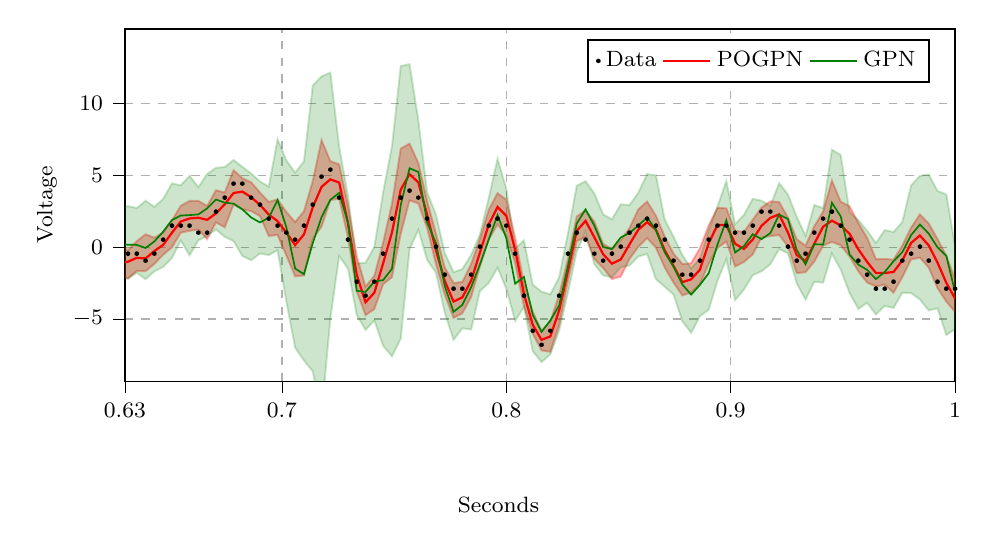
\begin{tikzpicture}
    \tikzstyle{every node}=[font=\footnotesize]
    \pgfplotsset{grid style={dashed,gray},
        width=1.0\columnwidth,
        height=0.5\columnwidth}
    \definecolor{darkgray176}{RGB}{176,176,176}
    \definecolor{green01270}{RGB}{0,127,0}

    \begin{axis}[
            tick align=outside,
            tick pos=left,
            % title={Prediction results for F2 sensor},
            x grid style={darkgray176},
            xtick={0.63, 0.7, 0.8, 0.9, 1},  % Custom x-tick positions
            % xticklabels={0.63, 0.7, Seconds, 0.9, 1.0},
            ytick={-5, 0, 5, 10},% Custom y-tick positions
            xlabel={Seconds},
            xlabel style={at={(axis description cs:0.45,-0.4)}, anchor=south},
            xmajorgrids,
            xmin=0.63, xmax=1,
            xtick style={color=black},
            y grid style={darkgray176},
            ylabel={Voltage},
            ylabel style={at={(axis description cs:-0.07,0.5)}, anchor=south},
            ymajorgrids,
            ymin=-9.35739350318909, ymax=15.2354862689972,
            ytick style={color=black},
            legend columns=3,
            legend pos=north east % Position of the legend
        ]
        \path [draw=red, fill=red, opacity=0.3]
        (axis cs:0.611764705882353,-1.3775120973587)
        --(axis cs:0.611764705882353,-3.78553867340088)
        --(axis cs:0.615686274509804,-3.19549036026001)
        --(axis cs:0.619607843137255,-2.60426354408264)
        --(axis cs:0.623529411764706,-1.99119591712952)
        --(axis cs:0.627450980392157,-1.90910744667053)
        --(axis cs:0.631372549019608,-2.1897029876709)
        --(axis cs:0.635294117647059,-1.65093731880188)
        --(axis cs:0.63921568627451,-1.66857504844666)
        --(axis cs:0.643137254901961,-1.16310608386993)
        --(axis cs:0.647058823529412,-0.520965099334717)
        --(axis cs:0.650980392156863,-0.00384068489074707)
        --(axis cs:0.654901960784314,1.0147705078125)
        --(axis cs:0.658823529411765,1.14194178581238)
        --(axis cs:0.662745098039216,1.23702788352966)
        --(axis cs:0.666666666666667,0.566851377487183)
        --(axis cs:0.670588235294118,1.73657321929932)
        --(axis cs:0.674509803921569,1.39279985427856)
        --(axis cs:0.67843137254902,2.97093152999878)
        --(axis cs:0.682352941176471,2.64094495773315)
        --(axis cs:0.686274509803922,2.51537942886353)
        --(axis cs:0.690196078431373,2.17144680023193)
        --(axis cs:0.694117647058824,0.788373947143555)
        --(axis cs:0.698039215686274,0.854525327682495)
        --(axis cs:0.701960784313725,-0.577107191085815)
        --(axis cs:0.705882352941176,-2.02998661994934)
        --(axis cs:0.709803921568627,-1.96817028522491)
        --(axis cs:0.713725490196078,0.586640357971191)
        --(axis cs:0.717647058823529,1.43421959877014)
        --(axis cs:0.72156862745098,3.28535842895508)
        --(axis cs:0.725490196078431,3.38800048828125)
        --(axis cs:0.729411764705882,0.693557262420654)
        --(axis cs:0.733333333333333,-3.0828058719635)
        --(axis cs:0.737254901960784,-4.73423767089844)
        --(axis cs:0.741176470588235,-4.30781078338623)
        --(axis cs:0.745098039215686,-2.57689571380615)
        --(axis cs:0.749019607843137,-2.08642768859863)
        --(axis cs:0.752941176470588,0.942610263824463)
        --(axis cs:0.756862745098039,3.2673454284668)
        --(axis cs:0.76078431372549,3.04598093032837)
        --(axis cs:0.764705882352941,1.33672547340393)
        --(axis cs:0.768627450980392,-1.17098462581635)
        --(axis cs:0.772549019607843,-3.30250310897827)
        --(axis cs:0.776470588235294,-4.92802906036377)
        --(axis cs:0.780392156862745,-4.60748958587646)
        --(axis cs:0.784313725490196,-3.46068263053894)
        --(axis cs:0.788235294117647,-1.32178997993469)
        --(axis cs:0.792156862745098,0.534637689590454)
        --(axis cs:0.796078431372549,1.58486413955688)
        --(axis cs:0.8,0.811280250549316)
        --(axis cs:0.803921568627451,-1.1207412481308)
        --(axis cs:0.807843137254902,-4.11320972442627)
        --(axis cs:0.811764705882353,-6.0285587310791)
        --(axis cs:0.815686274509804,-7.19171953201294)
        --(axis cs:0.819607843137255,-7.2888331413269)
        --(axis cs:0.823529411764706,-5.42310523986816)
        --(axis cs:0.827450980392157,-2.33326649665833)
        --(axis cs:0.831372549019608,0.414859771728516)
        --(axis cs:0.835294117647059,0.729306221008301)
        --(axis cs:0.83921568627451,-0.813742160797119)
        --(axis cs:0.843137254901961,-1.44217586517334)
        --(axis cs:0.847058823529412,-2.21199011802673)
        --(axis cs:0.850980392156863,-2.04721713066101)
        --(axis cs:0.854901960784314,-0.812328338623047)
        --(axis cs:0.858823529411765,0.0294883251190186)
        --(axis cs:0.862745098039216,0.637239694595337)
        --(axis cs:0.866666666666667,-0.0349938869476318)
        --(axis cs:0.870588235294118,-1.41949737071991)
        --(axis cs:0.874509803921569,-2.4594886302948)
        --(axis cs:0.87843137254902,-3.35607504844666)
        --(axis cs:0.882352941176471,-3.15800046920776)
        --(axis cs:0.886274509803922,-2.57187247276306)
        --(axis cs:0.890196078431372,-1.15262269973755)
        --(axis cs:0.894117647058823,-0.0438482761383057)
        --(axis cs:0.898039215686275,0.396376132965088)
        --(axis cs:0.901960784313726,-1.34793293476105)
        --(axis cs:0.905882352941176,-1.02713322639465)
        --(axis cs:0.909803921568627,-0.499524354934692)
        --(axis cs:0.913725490196078,0.685057640075684)
        --(axis cs:0.917647058823529,0.77232813835144)
        --(axis cs:0.92156862745098,0.85558009147644)
        --(axis cs:0.925490196078431,0.0534212589263916)
        --(axis cs:0.929411764705882,-1.80437088012695)
        --(axis cs:0.933333333333333,-1.74300646781921)
        --(axis cs:0.937254901960784,-0.995197296142578)
        --(axis cs:0.941176470588235,0.111906290054321)
        --(axis cs:0.945098039215686,0.372348785400391)
        --(axis cs:0.949019607843137,0.13739275932312)
        --(axis cs:0.952941176470588,-0.643450975418091)
        --(axis cs:0.956862745098039,-1.6729496717453)
        --(axis cs:0.96078431372549,-2.46090078353882)
        --(axis cs:0.964705882352941,-2.73789048194885)
        --(axis cs:0.968627450980392,-2.61531281471252)
        --(axis cs:0.972549019607843,-3.16955804824829)
        --(axis cs:0.976470588235294,-2.08453369140625)
        --(axis cs:0.980392156862745,-0.847957015037537)
        --(axis cs:0.984313725490196,-0.724214553833008)
        --(axis cs:0.988235294117647,-1.41829669475555)
        --(axis cs:0.992156862745098,-2.84473657608032)
        --(axis cs:0.996078431372549,-3.7876570224762)
        --(axis cs:1,-4.50478267669678)
        --(axis cs:1,-2.23178958892822)
        --(axis cs:1,-2.23178958892822)
        --(axis cs:0.996078431372549,-0.592119216918945)
        --(axis cs:0.992156862745098,0.57177734375)
        --(axis cs:0.988235294117647,1.6530933380127)
        --(axis cs:0.984313725490196,2.28956270217896)
        --(axis cs:0.980392156862745,1.37139344215393)
        --(axis cs:0.976470588235294,0.115371942520142)
        --(axis cs:0.972549019607843,-0.86380672454834)
        --(axis cs:0.968627450980392,-0.818130493164062)
        --(axis cs:0.964705882352941,-0.827772259712219)
        --(axis cs:0.96078431372549,0.65636944770813)
        --(axis cs:0.956862745098039,1.68610143661499)
        --(axis cs:0.952941176470588,2.86161708831787)
        --(axis cs:0.949019607843137,3.17119979858398)
        --(axis cs:0.945098039215686,4.64400815963745)
        --(axis cs:0.941176470588235,2.48467683792114)
        --(axis cs:0.937254901960784,1.47083187103271)
        --(axis cs:0.933333333333333,0.111169338226318)
        --(axis cs:0.929411764705882,0.561801433563232)
        --(axis cs:0.925490196078431,2.07613754272461)
        --(axis cs:0.92156862745098,3.14781761169434)
        --(axis cs:0.917647058823529,3.19638204574585)
        --(axis cs:0.913725490196078,2.76557922363281)
        --(axis cs:0.909803921568627,1.91688632965088)
        --(axis cs:0.905882352941176,1.06802368164062)
        --(axis cs:0.901960784313726,1.1446361541748)
        --(axis cs:0.898039215686275,2.71129941940308)
        --(axis cs:0.894117647058823,2.74595212936401)
        --(axis cs:0.890196078431372,1.52999830245972)
        --(axis cs:0.886274509803922,-0.0688066482543945)
        --(axis cs:0.882352941176471,-1.12141764163971)
        --(axis cs:0.87843137254902,-1.16305351257324)
        --(axis cs:0.874509803921569,-0.44484543800354)
        --(axis cs:0.870588235294118,0.749606609344482)
        --(axis cs:0.866666666666667,2.19831037521362)
        --(axis cs:0.862745098039216,3.18459939956665)
        --(axis cs:0.858823529411765,2.6448335647583)
        --(axis cs:0.854901960784314,1.34291577339172)
        --(axis cs:0.850980392156863,0.484196424484253)
        --(axis cs:0.847058823529412,-0.135904788970947)
        --(axis cs:0.843137254901961,0.246227502822876)
        --(axis cs:0.83921568627451,1.79609203338623)
        --(axis cs:0.835294117647059,2.56202745437622)
        --(axis cs:0.831372549019608,2.15173435211182)
        --(axis cs:0.827450980392157,-0.807169079780579)
        --(axis cs:0.823529411764706,-3.31553983688354)
        --(axis cs:0.819607843137255,-5.16366338729858)
        --(axis cs:0.815686274509804,-5.82039546966553)
        --(axis cs:0.811764705882353,-4.47896766662598)
        --(axis cs:0.807843137254902,-2.54403519630432)
        --(axis cs:0.803921568627451,0.674861431121826)
        --(axis cs:0.8,3.30196189880371)
        --(axis cs:0.796078431372549,3.76890707015991)
        --(axis cs:0.792156862745098,2.61391735076904)
        --(axis cs:0.788235294117647,0.591257572174072)
        --(axis cs:0.784313725490196,-1.17138087749481)
        --(axis cs:0.780392156862745,-2.41680192947388)
        --(axis cs:0.776470588235294,-2.49542117118835)
        --(axis cs:0.772549019607843,-1.40793800354004)
        --(axis cs:0.768627450980392,0.953491687774658)
        --(axis cs:0.764705882352941,3.21398973464966)
        --(axis cs:0.76078431372549,5.87122821807861)
        --(axis cs:0.756862745098039,7.21986103057861)
        --(axis cs:0.752941176470588,6.87029933929443)
        --(axis cs:0.749019607843137,3.04068279266357)
        --(axis cs:0.745098039215686,0.3219895362854)
        --(axis cs:0.741176470588235,-1.99327003955841)
        --(axis cs:0.737254901960784,-2.74070072174072)
        --(axis cs:0.733333333333333,-0.635098457336426)
        --(axis cs:0.729411764705882,2.91203022003174)
        --(axis cs:0.725490196078431,5.77520656585693)
        --(axis cs:0.72156862745098,5.99936389923096)
        --(axis cs:0.717647058823529,7.46705722808838)
        --(axis cs:0.713725490196078,4.6192569732666)
        --(axis cs:0.709803921568627,2.5088357925415)
        --(axis cs:0.705882352941176,1.74707412719727)
        --(axis cs:0.701960784313725,2.45908212661743)
        --(axis cs:0.698039215686274,3.33804750442505)
        --(axis cs:0.694117647058824,3.15559673309326)
        --(axis cs:0.690196078431373,3.81607151031494)
        --(axis cs:0.686274509803922,4.52596235275269)
        --(axis cs:0.682352941176471,4.80931949615479)
        --(axis cs:0.67843137254902,5.37073707580566)
        --(axis cs:0.674509803921569,3.81786251068115)
        --(axis cs:0.670588235294118,3.9695200920105)
        --(axis cs:0.666666666666667,2.87523412704468)
        --(axis cs:0.662745098039216,3.22832155227661)
        --(axis cs:0.658823529411765,3.2275071144104)
        --(axis cs:0.654901960784314,2.88368034362793)
        --(axis cs:0.650980392156863,1.87737989425659)
        --(axis cs:0.647058823529412,1.02051973342896)
        --(axis cs:0.643137254901961,0.665480136871338)
        --(axis cs:0.63921568627451,0.904106616973877)
        --(axis cs:0.635294117647059,0.427176713943481)
        --(axis cs:0.631372549019608,-0.213354349136353)
        --(axis cs:0.627450980392157,0.231562376022339)
        --(axis cs:0.623529411764706,-0.13664174079895)
        --(axis cs:0.619607843137255,-0.515468716621399)
        --(axis cs:0.615686274509804,-0.952359318733215)
        --(axis cs:0.611764705882353,-1.3775120973587)
        --cycle;

        \path [draw=green01270, fill=green01270, opacity=0.2]
        (axis cs:0.611764705882353,-2.07992744445801)
        --(axis cs:0.611764705882353,-7.00844955444336)
        --(axis cs:0.615686274509804,-4.85382175445557)
        --(axis cs:0.619607843137255,-3.36874151229858)
        --(axis cs:0.623529411764706,-2.35852074623108)
        --(axis cs:0.627450980392157,-2.17008543014526)
        --(axis cs:0.631372549019608,-2.17208671569824)
        --(axis cs:0.635294117647059,-1.78458285331726)
        --(axis cs:0.63921568627451,-2.23014783859253)
        --(axis cs:0.643137254901961,-1.68191051483154)
        --(axis cs:0.647058823529412,-1.36969888210297)
        --(axis cs:0.650980392156863,-0.760860562324524)
        --(axis cs:0.654901960784314,0.470986604690552)
        --(axis cs:0.658823529411765,-0.561428189277649)
        --(axis cs:0.662745098039216,0.478718996047974)
        --(axis cs:0.666666666666667,0.784774780273438)
        --(axis cs:0.670588235294118,1.23616886138916)
        --(axis cs:0.674509803921569,0.725908517837524)
        --(axis cs:0.67843137254902,0.430788993835449)
        --(axis cs:0.682352941176471,-0.604689598083496)
        --(axis cs:0.686274509803922,-0.907554507255554)
        --(axis cs:0.690196078431373,-0.437394499778748)
        --(axis cs:0.694117647058824,-0.549601078033447)
        --(axis cs:0.698039215686274,-0.201310873031616)
        --(axis cs:0.701960784313725,-3.77312183380127)
        --(axis cs:0.705882352941176,-6.99996137619019)
        --(axis cs:0.709803921568627,-7.89466381072998)
        --(axis cs:0.713725490196078,-8.65226459503174)
        --(axis cs:0.717647058823529,-11.6528091430664)
        --(axis cs:0.72156862745098,-4.97210884094238)
        --(axis cs:0.725490196078431,-0.62409496307373)
        --(axis cs:0.729411764705882,-1.47812283039093)
        --(axis cs:0.733333333333333,-4.72654390335083)
        --(axis cs:0.737254901960784,-5.75822257995605)
        --(axis cs:0.741176470588235,-5.10161209106445)
        --(axis cs:0.745098039215686,-6.86520051956177)
        --(axis cs:0.749019607843137,-7.60363817214966)
        --(axis cs:0.752941176470588,-6.3772120475769)
        --(axis cs:0.756862745098039,-0.129380226135254)
        --(axis cs:0.76078431372549,1.20826244354248)
        --(axis cs:0.764705882352941,-0.881188988685608)
        --(axis cs:0.768627450980392,-1.77494597434998)
        --(axis cs:0.772549019607843,-4.55769872665405)
        --(axis cs:0.776470588235294,-6.45461654663086)
        --(axis cs:0.780392156862745,-5.65339851379395)
        --(axis cs:0.784313725490196,-5.73344230651855)
        --(axis cs:0.788235294117647,-3.05585885047913)
        --(axis cs:0.792156862745098,-2.49463176727295)
        --(axis cs:0.796078431372549,-1.4203165769577)
        --(axis cs:0.8,-2.89834856987)
        --(axis cs:0.803921568627451,-5.13593482971191)
        --(axis cs:0.807843137254902,-4.1600456237793)
        --(axis cs:0.811764705882353,-7.25151634216309)
        --(axis cs:0.815686274509804,-8.00917625427246)
        --(axis cs:0.819607843137255,-7.46355485916138)
        --(axis cs:0.823529411764706,-5.82308101654053)
        --(axis cs:0.827450980392157,-3.17450213432312)
        --(axis cs:0.831372549019608,-0.287919282913208)
        --(axis cs:0.835294117647059,1.06624269485474)
        --(axis cs:0.83921568627451,-1.18726575374603)
        --(axis cs:0.843137254901961,-1.95926117897034)
        --(axis cs:0.847058823529412,-2.10349225997925)
        --(axis cs:0.850980392156863,-1.39311492443085)
        --(axis cs:0.854901960784314,-1.26745975017548)
        --(axis cs:0.858823529411765,-0.644472718238831)
        --(axis cs:0.862745098039216,-0.470396161079407)
        --(axis cs:0.866666666666667,-2.22762680053711)
        --(axis cs:0.870588235294118,-2.75909423828125)
        --(axis cs:0.874509803921569,-3.29242992401123)
        --(axis cs:0.87843137254902,-5.15087699890137)
        --(axis cs:0.882352941176471,-5.97006988525391)
        --(axis cs:0.886274509803922,-4.80386352539062)
        --(axis cs:0.890196078431372,-4.35644006729126)
        --(axis cs:0.894117647058823,-2.32477378845215)
        --(axis cs:0.898039215686275,-0.829452157020569)
        --(axis cs:0.901960784313726,-3.68932151794434)
        --(axis cs:0.905882352941176,-2.94063639640808)
        --(axis cs:0.909803921568627,-1.94849920272827)
        --(axis cs:0.913725490196078,-1.67658150196075)
        --(axis cs:0.917647058823529,-1.18600499629974)
        --(axis cs:0.92156862745098,-0.127111315727234)
        --(axis cs:0.925490196078431,-0.423864722251892)
        --(axis cs:0.929411764705882,-2.51412296295166)
        --(axis cs:0.933333333333333,-3.64739179611206)
        --(axis cs:0.937254901960784,-2.40362143516541)
        --(axis cs:0.941176470588235,-2.4700345993042)
        --(axis cs:0.945098039215686,-0.435311555862427)
        --(axis cs:0.949019607843137,-1.55577170848846)
        --(axis cs:0.952941176470588,-3.18346405029297)
        --(axis cs:0.956862745098039,-4.29701471328735)
        --(axis cs:0.96078431372549,-3.87511301040649)
        --(axis cs:0.964705882352941,-4.68247222900391)
        --(axis cs:0.968627450980392,-4.09334087371826)
        --(axis cs:0.972549019607843,-4.2289776802063)
        --(axis cs:0.976470588235294,-3.17436504364014)
        --(axis cs:0.980392156862745,-3.18987131118774)
        --(axis cs:0.984313725490196,-3.63956689834595)
        --(axis cs:0.988235294117647,-4.4048433303833)
        --(axis cs:0.992156862745098,-4.25834035873413)
        --(axis cs:0.996078431372549,-6.11209058761597)
        --(axis cs:1,-5.71347332000732)
        --(axis cs:1,0.0671453475952148)
        --(axis cs:1,0.0671453475952148)
        --(axis cs:0.996078431372549,3.68257474899292)
        --(axis cs:0.992156862745098,3.92190217971802)
        --(axis cs:0.988235294117647,5.07468795776367)
        --(axis cs:0.984313725490196,4.96925783157349)
        --(axis cs:0.980392156862745,4.30890655517578)
        --(axis cs:0.976470588235294,1.75945389270782)
        --(axis cs:0.972549019607843,1.06043219566345)
        --(axis cs:0.968627450980392,1.19268035888672)
        --(axis cs:0.964705882352941,0.290719032287598)
        --(axis cs:0.96078431372549,1.15779757499695)
        --(axis cs:0.956862745098039,1.89983236789703)
        --(axis cs:0.952941176470588,2.44486474990845)
        --(axis cs:0.949019607843137,6.42357063293457)
        --(axis cs:0.945098039215686,6.80671787261963)
        --(axis cs:0.941176470588235,2.72088766098022)
        --(axis cs:0.937254901960784,2.94576215744019)
        --(axis cs:0.933333333333333,0.798133730888367)
        --(axis cs:0.929411764705882,2.11707162857056)
        --(axis cs:0.925490196078431,3.67766332626343)
        --(axis cs:0.92156862745098,4.46824789047241)
        --(axis cs:0.917647058823529,2.87133622169495)
        --(axis cs:0.913725490196078,3.24577856063843)
        --(axis cs:0.909803921568627,3.37059259414673)
        --(axis cs:0.905882352941176,2.26035213470459)
        --(axis cs:0.901960784313726,1.60065650939941)
        --(axis cs:0.898039215686275,4.61139917373657)
        --(axis cs:0.894117647058823,2.85120296478271)
        --(axis cs:0.890196078431372,1.19247388839722)
        --(axis cs:0.886274509803922,-0.798310518264771)
        --(axis cs:0.882352941176471,-1.47946405410767)
        --(axis cs:0.87843137254902,-0.533737063407898)
        --(axis cs:0.874509803921569,0.730034470558167)
        --(axis cs:0.870588235294118,1.93347382545471)
        --(axis cs:0.866666666666667,5.01113843917847)
        --(axis cs:0.862745098039216,5.09384536743164)
        --(axis cs:0.858823529411765,3.80219650268555)
        --(axis cs:0.854901960784314,2.93519234657288)
        --(axis cs:0.850980392156863,2.99006080627441)
        --(axis cs:0.847058823529412,1.94261419773102)
        --(axis cs:0.843137254901961,2.29301118850708)
        --(axis cs:0.83921568627451,3.74940800666809)
        --(axis cs:0.835294117647059,4.60163545608521)
        --(axis cs:0.831372549019608,4.28139781951904)
        --(axis cs:0.827450980392157,0.954022884368896)
        --(axis cs:0.823529411764706,-2.09404325485229)
        --(axis cs:0.819607843137255,-3.28287124633789)
        --(axis cs:0.815686274509804,-3.10021567344666)
        --(axis cs:0.811764705882353,-2.60481548309326)
        --(axis cs:0.807843137254902,0.474199533462524)
        --(axis cs:0.803921568627451,-0.0903904438018799)
        --(axis cs:0.8,4.0727014541626)
        --(axis cs:0.796078431372549,6.16085910797119)
        --(axis cs:0.792156862745098,3.42145872116089)
        --(axis cs:0.788235294117647,0.902291178703308)
        --(axis cs:0.784313725490196,-0.532938003540039)
        --(axis cs:0.780392156862745,-1.52215814590454)
        --(axis cs:0.776470588235294,-1.7388219833374)
        --(axis cs:0.772549019607843,-0.396997451782227)
        --(axis cs:0.768627450980392,2.27793169021606)
        --(axis cs:0.764705882352941,3.81951785087585)
        --(axis cs:0.76078431372549,8.8552770614624)
        --(axis cs:0.756862745098039,12.7528762817383)
        --(axis cs:0.752941176470588,12.6306190490723)
        --(axis cs:0.749019607843137,7.03158617019653)
        --(axis cs:0.745098039215686,3.8331139087677)
        --(axis cs:0.741176470588235,0.0201380252838135)
        --(axis cs:0.737254901960784,-1.07146155834198)
        --(axis cs:0.733333333333333,-1.14122653007507)
        --(axis cs:0.729411764705882,3.58289051055908)
        --(axis cs:0.725490196078431,7.00733470916748)
        --(axis cs:0.72156862745098,12.1671781539917)
        --(axis cs:0.717647058823529,11.9081325531006)
        --(axis cs:0.713725490196078,11.2696352005005)
        --(axis cs:0.709803921568627,5.98610973358154)
        --(axis cs:0.705882352941176,5.19701099395752)
        --(axis cs:0.701960784313725,6.04594564437866)
        --(axis cs:0.698039215686274,7.52167510986328)
        --(axis cs:0.694117647058824,4.22802877426147)
        --(axis cs:0.690196078431373,4.58402729034424)
        --(axis cs:0.686274509803922,5.13973426818848)
        --(axis cs:0.682352941176471,5.60300970077515)
        --(axis cs:0.67843137254902,6.08319330215454)
        --(axis cs:0.674509803921569,5.58561944961548)
        --(axis cs:0.670588235294118,5.53740978240967)
        --(axis cs:0.666666666666667,5.10034370422363)
        --(axis cs:0.662745098039216,4.18194770812988)
        --(axis cs:0.658823529411765,4.98029470443726)
        --(axis cs:0.654901960784314,4.31359434127808)
        --(axis cs:0.650980392156863,4.45203018188477)
        --(axis cs:0.647058823529412,3.36548089981079)
        --(axis cs:0.643137254901961,2.81954455375671)
        --(axis cs:0.63921568627451,3.24272680282593)
        --(axis cs:0.635294117647059,2.7318434715271)
        --(axis cs:0.631372549019608,2.86524486541748)
        --(axis cs:0.627450980392157,2.6537971496582)
        --(axis cs:0.623529411764706,1.94467067718506)
        --(axis cs:0.619607843137255,0.489394664764404)
        --(axis cs:0.615686274509804,-1.30745720863342)
        --(axis cs:0.611764705882353,-2.07992744445801)
        --cycle;
        \addplot [semithick, black, mark=asterisk, mark size=0.8, mark options={solid}, only marks]
        table {%
                0.611764705882353 -2.40100002288818
                0.615686274509804 -2.40100002288818
                0.619607843137255 -2.40100002288818
                0.623529411764706 -1.42400002479553
                0.627450980392157 -0.935999989509583
                0.631372549019608 -0.447999954223633
                0.635294117647059 -0.447999954223633
                0.63921568627451 -0.935999989509583
                0.643137254901961 -0.447999954223633
                0.647058823529412 0.529000043869019
                0.650980392156863 1.50599980354309
                0.654901960784314 1.50599980354309
                0.658823529411765 1.50599980354309
                0.662745098039216 1.01699995994568
                0.666666666666667 1.01699995994568
                0.670588235294118 2.48200011253357
                0.674509803921569 3.45899987220764
                0.67843137254902 4.43499946594238
                0.682352941176471 4.43499946594238
                0.686274509803922 3.45899987220764
                0.690196078431373 2.97000002861023
                0.694117647058824 1.99399971961975
                0.698039215686274 1.50599980354309
                0.701960784313725 1.01699995994568
                0.705882352941176 0.529000043869019
                0.709803921568627 1.50599980354309
                0.713725490196078 2.97000002861023
                0.717647058823529 4.92399978637695
                0.72156862745098 5.41199970245361
                0.725490196078431 3.45899987220764
                0.729411764705882 0.529000043869019
                0.733333333333333 -2.40100002288818
                0.737254901960784 -3.37700009346008
                0.741176470588235 -2.40100002288818
                0.745098039215686 -0.447999954223633
                0.749019607843137 1.99399971961975
                0.752941176470588 3.45899987220764
                0.756862745098039 3.9469997882843
                0.76078431372549 3.45899987220764
                0.764705882352941 1.99399971961975
                0.768627450980392 0.0409998893737793
                0.772549019607843 -1.91199994087219
                0.776470588235294 -2.88899993896484
                0.780392156862745 -2.88899993896484
                0.784313725490196 -1.91199994087219
                0.788235294117647 0.0409998893737793
                0.792156862745098 1.50599980354309
                0.796078431372549 1.99399971961975
                0.8 1.50599980354309
                0.803921568627451 -0.447999954223633
                0.807843137254902 -3.37700009346008
                0.811764705882353 -5.81899976730347
                0.815686274509804 -6.79500007629395
                0.819607843137255 -5.81899976730347
                0.823529411764706 -3.37700009346008
                0.827450980392157 -0.447999954223633
                0.831372549019608 1.01699995994568
                0.835294117647059 0.529000043869019
                0.83921568627451 -0.447999954223633
                0.843137254901961 -0.935999989509583
                0.847058823529412 -0.447999954223633
                0.850980392156863 0.0409998893737793
                0.854901960784314 1.01699995994568
                0.858823529411765 1.50599980354309
                0.862745098039216 1.99399971961975
                0.866666666666667 1.50599980354309
                0.870588235294118 0.529000043869019
                0.874509803921569 -0.935999989509583
                0.87843137254902 -1.91199994087219
                0.882352941176471 -1.91199994087219
                0.886274509803922 -0.935999989509583
                0.890196078431372 0.529000043869019
                0.894117647058823 1.50599980354309
                0.898039215686275 1.50599980354309
                0.901960784313726 1.01699995994568
                0.905882352941176 1.01699995994568
                0.909803921568627 1.50599980354309
                0.913725490196078 2.48200011253357
                0.917647058823529 2.48200011253357
                0.92156862745098 1.50599980354309
                0.925490196078431 0.0409998893737793
                0.929411764705882 -0.935999989509583
                0.933333333333333 -0.447999954223633
                0.937254901960784 1.01699995994568
                0.941176470588235 1.99399971961975
                0.945098039215686 2.48200011253357
                0.949019607843137 1.50599980354309
                0.952941176470588 0.529000043869019
                0.956862745098039 -0.935999989509583
                0.96078431372549 -1.91199994087219
                0.964705882352941 -2.88899993896484
                0.968627450980392 -2.88899993896484
                0.972549019607843 -2.40100002288818
                0.976470588235294 -0.935999989509583
                0.980392156862745 -0.447999954223633
                0.984313725490196 0.0409998893737793
                0.988235294117647 -0.935999989509583
                0.992156862745098 -2.40100002288818
                0.996078431372549 -2.88899993896484
                1 -2.88899993896484
            };\addlegendentry{Data}
        \addplot [thick, red]
        table {%
                0.611764705882353 -2.44729900360107
                0.615686274509804 -2.06386113166809
                0.619607843137255 -1.80806136131287
                0.623529411764706 -1.24518382549286
                0.627450980392157 -1.12641966342926
                0.631372549019608 -1.00942492485046
                0.635294117647059 -0.737217605113983
                0.63921568627451 -0.778968393802643
                0.643137254901961 -0.263900458812714
                0.647058823529412 0.164565652608871
                0.650980392156863 1.01316750049591
                0.654901960784314 1.79144394397736
                0.658823529411765 2.00494265556335
                0.662745098039216 2.0552966594696
                0.666666666666667 1.91173684597015
                0.670588235294118 2.35817193984985
                0.674509803921569 3.00009298324585
                0.67843137254902 3.77913570404053
                0.682352941176471 3.87787890434265
                0.686274509803922 3.48751068115234
                0.690196078431373 2.95148706436157
                0.694117647058824 2.27939009666443
                0.698039215686274 1.81683552265167
                0.701960784313725 1.01747858524323
                0.705882352941176 0.150215893983841
                0.709803921568627 0.892119348049164
                0.713725490196078 2.78885865211487
                0.717647058823529 4.20781517028809
                0.72156862745098 4.73084259033203
                0.725490196078431 4.50930309295654
                0.729411764705882 1.70955896377563
                0.733333333333333 -1.93018996715546
                0.737254901960784 -3.83528542518616
                0.741176470588235 -3.16600584983826
                0.745098039215686 -1.11889100074768
                0.749019607843137 1.03088080883026
                0.752941176470588 4.0189733505249
                0.756862745098039 5.09354209899902
                0.76078431372549 4.51752376556396
                0.764705882352941 2.25577831268311
                0.768627450980392 -0.208552554249763
                0.772549019607843 -2.35021543502808
                0.776470588235294 -3.78770589828491
                0.780392156862745 -3.49568557739258
                0.784313725490196 -2.32468771934509
                0.788235294117647 -0.373786151409149
                0.792156862745098 1.59017598628998
                0.796078431372549 2.80256772041321
                0.8 2.18350434303284
                0.803921568627451 -0.178723722696304
                0.807843137254902 -3.26432275772095
                0.811764705882353 -5.39990663528442
                0.815686274509804 -6.45723819732666
                0.819607843137255 -6.21320581436157
                0.823529411764706 -4.41227149963379
                0.827450980392157 -1.64686834812164
                0.831372549019608 1.14627802371979
                0.835294117647059 1.83653199672699
                0.83921568627451 0.693766176700592
                0.843137254901961 -0.48693573474884
                0.847058823529412 -1.14362967014313
                0.850980392156863 -0.855408787727356
                0.854901960784314 0.207694917917252
                0.858823529411765 1.22590982913971
                0.862745098039216 1.74730634689331
                0.866666666666667 1.22668242454529
                0.870588235294118 -0.215356960892677
                0.874509803921569 -1.30756902694702
                0.87843137254902 -2.43179297447205
                0.882352941176471 -2.23801207542419
                0.886274509803922 -1.56264078617096
                0.890196078431372 0.290053427219391
                0.894117647058823 1.55589234828949
                0.898039215686275 1.5351140499115
                0.901960784313726 0.244135662913322
                0.905882352941176 -0.118965625762939
                0.909803921568627 0.542053580284119
                0.913725490196078 1.49422788619995
                0.917647058823529 2.04629731178284
                0.92156862745098 2.28854918479919
                0.925490196078431 1.02471566200256
                0.929411764705882 -0.540462613105774
                0.933333333333333 -0.960569083690643
                0.937254901960784 0.249364912509918
                0.941176470588235 1.4279488325119
                0.945098039215686 1.85232126712799
                0.949019607843137 1.52062368392944
                0.952941176470588 0.940244913101196
                0.956862745098039 -0.144238203763962
                0.96078431372549 -1.02084076404572
                0.964705882352941 -1.79671967029572
                0.968627450980392 -1.79569792747498
                0.972549019607843 -1.72365212440491
                0.976470588235294 -0.928638577461243
                0.980392156862745 0.300802111625671
                0.984313725490196 0.815456032752991
                0.988235294117647 0.130474150180817
                0.992156862745098 -1.07184219360352
                0.996078431372549 -2.47789216041565
                1 -3.58779144287109
            };\addlegendentry{POGPN}
        \addplot [semithick, green01270]
        table {%
                0.611764705882353 -3.92067313194275
                0.615686274509804 -3.2660083770752
                0.619607843137255 -1.27702152729034
                0.623529411764706 0.0556083098053932
                0.627450980392157 0.232553899288177
                0.631372549019608 0.173902735114098
                0.635294117647059 0.163662552833557
                0.63921568627451 -0.0514964163303375
                0.643137254901961 0.405160993337631
                0.647058823529412 1.08335494995117
                0.650980392156863 1.89663147926331
                0.654901960784314 2.20957469940186
                0.658823529411765 2.23975872993469
                0.662745098039216 2.28995966911316
                0.666666666666667 2.70662593841553
                0.670588235294118 3.32468628883362
                0.674509803921569 3.10654973983765
                0.67843137254902 3.03907084465027
                0.682352941176471 2.64044523239136
                0.686274509803922 2.07396602630615
                0.690196078431373 1.72791433334351
                0.694117647058824 2.05307292938232
                0.698039215686274 3.28956365585327
                0.701960784313725 1.3900431394577
                0.705882352941176 -1.48941373825073
                0.709803921568627 -1.87544322013855
                0.713725490196078 0.285975277423859
                0.717647058823529 2.10237622261047
                0.72156862745098 3.3069314956665
                0.725490196078431 3.78715753555298
                0.729411764705882 1.71219968795776
                0.733333333333333 -3.03442740440369
                0.737254901960784 -3.11346673965454
                0.741176470588235 -2.3995418548584
                0.745098039215686 -2.28784465789795
                0.749019607843137 -1.49938690662384
                0.752941176470588 2.94682645797729
                0.756862745098039 5.50504207611084
                0.76078431372549 5.24793863296509
                0.764705882352941 1.72702288627625
                0.768627450980392 0.291814535856247
                0.772549019607843 -2.70644736289978
                0.776470588235294 -4.50002241134644
                0.780392156862745 -4.0185399055481
                0.784313725490196 -2.77829384803772
                0.788235294117647 -1.19785678386688
                0.792156862745098 0.543276071548462
                0.796078431372549 2.24091839790344
                0.8 0.626825153827667
                0.803921568627451 -2.537264585495
                0.807843137254902 -2.07123398780823
                0.811764705882353 -4.70518350601196
                0.815686274509804 -5.89906787872314
                0.819607843137255 -5.10353469848633
                0.823529411764706 -4.06041383743286
                0.827450980392157 -1.32311034202576
                0.831372549019608 1.64632022380829
                0.835294117647059 2.63942718505859
                0.83921568627451 1.50559556484222
                0.843137254901961 0.0139899300411344
                0.847058823529412 -0.126856714487076
                0.850980392156863 0.681717932224274
                0.854901960784314 0.993287205696106
                0.858823529411765 1.51723957061768
                0.862745098039216 2.08137989044189
                0.866666666666667 1.18420720100403
                0.870588235294118 -0.36256530880928
                0.874509803921569 -1.35062420368195
                0.87843137254902 -2.59938144683838
                0.882352941176471 -3.30386686325073
                0.886274509803922 -2.62303948402405
                0.890196078431372 -1.80651795864105
                0.894117647058823 0.196709305047989
                0.898039215686275 1.8824428319931
                0.901960784313726 -0.367957502603531
                0.905882352941176 0.0791754573583603
                0.909803921568627 0.907748818397522
                0.913725490196078 0.564049005508423
                0.917647058823529 0.981567740440369
                0.92156862745098 2.27241945266724
                0.925490196078431 1.96953821182251
                0.929411764705882 -0.196025803685188
                0.933333333333333 -1.1901650428772
                0.937254901960784 0.209711909294128
                0.941176470588235 0.188728556036949
                0.945098039215686 3.09708189964294
                0.949019607843137 2.14360880851746
                0.952941176470588 -0.50410932302475
                0.956862745098039 -1.20587968826294
                0.96078431372549 -1.57866728305817
                0.964705882352941 -2.21905732154846
                0.968627450980392 -1.72117710113525
                0.972549019607843 -0.976755857467651
                0.976470588235294 -0.343840062618256
                0.980392156862745 0.849320828914642
                0.984313725490196 1.58255314826965
                0.988235294117647 0.94932746887207
                0.992156862745098 -0.00475416192784905
                0.996078431372549 -0.60159295797348
                1 -3.14249110221863
            };\addlegendentry{GPN}
    \end{axis}

\end{tikzpicture}

            % \includegraphics{figures/popgn_eeg_pred.pdf}
            \caption{Prediction results for F2 sensor from EEG dataset.}
            \label{fig:eeg_pred}
      \end{subfigure}
      \caption{Structure of POGPN for EEG dataset in Figure~\ref{fig:eeg_dag}. Figure~\ref{fig:eeg_pred} shows prediction results for sensor F2 using POGPN-AL (PLL) and GPN with a similar concept as described by Figure~\ref{fig:toy_process_gpn}.} % Overall caption for the figure
      \label{fig:eeg_combined} % Overall label for the figure
      \vspace{-1em}
\end{figure}

\begin{table}[h]
      % Reduce the default column padding for the enclosed tables.
      \setlength{\tabcolsep}{4pt}
      \centering
      % Constrain the table width to fit within a single column
      \begin{tabular}{@{}c@{}}
            % First sub-table
            \begin{tabular}{@{\hskip 0pt}lcccc@{\hskip 0pt}}
                  \toprule
                  Model & IGP\textsuperscript{\textdagger} & SLFM\textsuperscript{\textdagger} & GPAR-NL\textsuperscript{\textdagger} & POGPN-AL (PLL) \\
                  \midrule
                  SMSE  &
                  1.75  &
                  1.06  &
                  0.26  &
                  \textbf{0.24}
                  \\
                  MLL   &
                  2.60  & 4.00                             & 1.63                              & 1.04
                  % $\pm$0.11
                  \\
                  \bottomrule
            \end{tabular}
            \\[2em] % Add vertical spacing between sub-tables

            % Second sub-table
            \begin{tabular}{@{\hskip 0pt}lcc@{\hskip 0pt}}
                  \toprule
                  Model & POGPN-NL (PLL) & POGPN-AL (ELBO) \\
                  \midrule
                  SMSE  & 0.28           & 0.31            \\
                  MLL   & \textbf{0.18}  & 1.40            \\
                  \bottomrule
            \end{tabular}
      \end{tabular}
      \caption{Prediction results for EEG dataset of different models. Standardized mean squared error (SMSE) and Mean Log Loss (MLL)~\cite{rasmussen2003gaussian} comparison (lower is better). Models marked with \textsuperscript{\textdagger} indicate cited results from~\cite{requeima2019gaussian}.}
      \vspace{-1em}
\end{table}
% \vspace{-1em}
Inducing locations are in the "Time" domain and kept the same as the total time steps (256 points) as used by~\cite{requeima2019gaussian} and remain constant throughout the training process. For evaluation, the values are standardized before training and transformed back before prediction evaluation. POGPN consistently outperforms GPAR, showing significant improvements in SMSE and MLL. The results demonstrate the robustness of POGN against process stochasticity and the potential for even better confidence intervals, as shown in Figure~\ref{fig:eeg_pred}.

\textbf{Synthetic experiment.} We use the synthetic experiment from~\cite{requeima2019gaussian} but change it to have categorical observations to test the performance of POGPN for non-Gaussian noise along with categorical and continuous observations from subprocesses. Since the existing GPNs cannot incorporate categorical intermediate observations, we compare against DGP with the same layer structure but without intermediate subprocess likelihoods. For $x\in[0, 1]$, the system is described as
\begin{align*}
      f_{1}(x)
       & = -\frac{\sin\!\bigl(10\pi\,(x + 1)\bigr)}{2x + 1} - x^{4}           \\
      f_{2}(x)
       & = \cos^{2}\!\bigl(f_{1}(x)\bigr) + \sin(3x),                         \\
      f_{3}(x)
       & =\begin{cases}
                f_{2}(x)\,f_{1}(x)^{2} + 3\,x - 2.5, & \text{if } f_{2}(x) < 1.5,   \\
                f_{2}(x)\,f_{1}(x)^{2} + 3\,x + 2.5, & \text{if } f_{2}(x) \ge 1.5,
          \end{cases}
\end{align*}
and the intermediate observations are defined as
\begin{align*}
      y_{1} & = f_{1}(x) + \delta_{\text{obs}}, \\
      y_{2} & =
      \begin{cases}
            0, & \text{if } f_{2}(x) < 1.5,   \\
            1, & \text{if } f_{2}(x) \ge 1.5,
      \end{cases}
\end{align*}
where final output $y_3=f_3 + \delta_{\text{obs}}$ and $\delta_{\text{obs}} \sim \mathcal{N}(0, 0.1)$.
\begin{figure}[ht]
      \centering
      \begin{subfigure}[t]{\columnwidth}
            \centering
            % \tikzset{every picture/.style={line width=0.7pt}} % Set default line width
% \begin{tikzpicture}[node distance=10mm and 10mm,
%             process/.style={circle, draw, minimum size=10mm, align=center, inner sep=0.5pt},
%             every node/.style={font=\footnotesize},
%             arr/.style={-Stealth},
%             obs/.style={circle, draw, fill=gray!30, minimum size=6.5mm, align=center, inner sep=0.5pt}
%       ]
%       % Define nodes
%       \node[process] (x) {$x$};
%       \node[process] (f1) [above=of x] {$f^{(1)}$};
%       \node[process] (f2) [right=of f1] {$f^{(2)}$};
%       \node[process] (f3) [below=of f2] {$f^{(3)}$};

%       \draw[arr] (x) -- (f1);
%       \draw[arr] (x) -- (f2);
%       \draw[arr] (f1) -- (f2);
%       \draw[arr] (x) -- (f3);
%       \draw[arr] (f1) -- (f3);
%       \draw[arr] (f2) -- (f3);

% \end{tikzpicture}
\begin{tikzpicture}[
        node distance=8mm and 8mm,       % Reduced spacing
        process/.style={circle, draw, minimum size=8mm, align=center, inner sep=0.5pt},
        every node/.style={font=\scriptsize},     % Slightly smaller font
        arr/.style={-Stealth}
    ]

    % Nodes in one horizontal line
    \node[process] (x) {$x$};
    \node[process, right=of x] (f1) {$f^{(1)}$};
    \node[process, right=of f1] (f2) {$f^{(2)}$};
    \node[process, right=of f2] (f3) {$f^{(3)}$};

    % Straight arrows
    \draw[arr] (x) -- (f1);
    \draw[arr] (f1) -- (f2);
    \draw[arr] (f2) -- (f3);

    % Curved arrows with reduced bends
    \draw[arr, bend left=23]  (x) to (f2);
    \draw[arr, bend left=25]  (x) to (f3);
    \draw[arr, bend right=23] (f1) to (f3);

\end{tikzpicture}
            \caption{Structure of POGPN for synthetic experiment with Gaussian likelihood for $f^{(1)}$ and $f^{(3)}$, and Bernoulli likelihood for $f^{(2)}$.}
            % \vspace{-1em}
            \label{fig:synthetic_dag}
      \end{subfigure}
      \hfill
      \begin{subfigure}[t]{\columnwidth}
            \centering
            % This file was created with tikzplotlib v0.10.1.
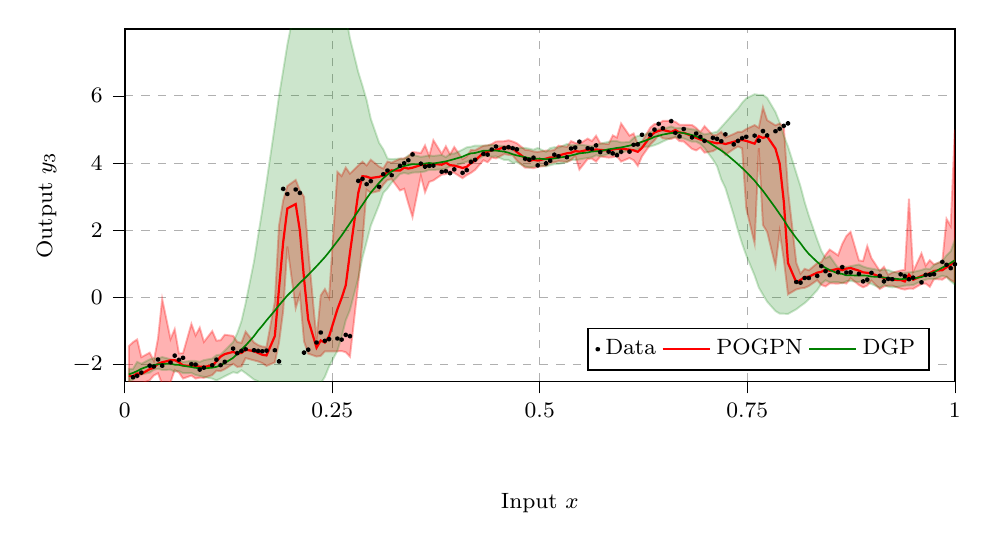
\begin{tikzpicture}
    \tikzstyle{every node}=[font=\footnotesize]
    \pgfplotsset{grid style={dashed,gray},
        width=1.0\columnwidth,
        height=0.5\columnwidth}
    \definecolor{darkgray176}{RGB}{176,176,176}
    \definecolor{green01270}{RGB}{0,127,0}

    \begin{axis}[
            tick align=outside,
            tick pos=left,
            % title={Prediction results for F2 sensor},
            x grid style={darkgray176},
            xtick={0.0, 0.25, 0.5, 0.75, 1},  % Custom x-tick positions
            % xticklabels={0.63, 0.7, Seconds, 0.9, 1.0},
            ytick={-2, 0, 2, 4, 6},% Custom y-tick positions
            xlabel={Input $x$},
            xlabel style={at={(axis description cs:0.5,-0.4)}, anchor=south},
            xmajorgrids,
            xmin=0.0, xmax=1.0,
            xtick style={color=black},
            y grid style={darkgray176},
            ylabel={Output $y_{3}$},
            ylabel style={at={(axis description cs:-0.07,0.5)}, anchor=south},
            ymajorgrids,
            ymin=-2.5, ymax=8,
            ytick style={color=black},
            legend columns=3,
            legend pos=south east % Position of the legend
        ]
        \path [draw=red, fill=red, opacity=0.3]
        (axis cs:0.0050251256281407,-1.45085072517395)
        --(axis cs:0.0050251256281407,-2.6801655292511)
        --(axis cs:0.0100502512562814,-2.82710003852844)
        --(axis cs:0.0150753768844221,-2.66949772834778)
        --(axis cs:0.0201005025125628,-2.56169486045837)
        --(axis cs:0.0301507537688442,-2.46433043479919)
        --(axis cs:0.0351758793969849,-2.32039999961853)
        --(axis cs:0.0402010050251256,-2.25510334968567)
        --(axis cs:0.0452261306532663,-2.58824229240417)
        --(axis cs:0.0552763819095477,-2.52013611793518)
        --(axis cs:0.0603015075376884,-2.15734171867371)
        --(axis cs:0.0653266331658292,-2.23198485374451)
        --(axis cs:0.0703517587939698,-2.41198563575745)
        --(axis cs:0.0804020100502513,-2.3244092464447)
        --(axis cs:0.085427135678392,-2.41153883934021)
        --(axis cs:0.0904522613065327,-2.38634705543518)
        --(axis cs:0.0954773869346734,-2.39137101173401)
        --(axis cs:0.105527638190955,-2.30893397331238)
        --(axis cs:0.110552763819095,-2.17822766304016)
        --(axis cs:0.115577889447236,-2.18981003761292)
        --(axis cs:0.120603015075377,-2.1345522403717)
        --(axis cs:0.130653266331658,-1.97399044036865)
        --(axis cs:0.135678391959799,-2.06450963020325)
        --(axis cs:0.14070351758794,-2.05153059959412)
        --(axis cs:0.14572864321608,-1.80440878868103)
        --(axis cs:0.155778894472362,-1.87098574638367)
        --(axis cs:0.160804020100503,-1.90363168716431)
        --(axis cs:0.165829145728643,-1.95318865776062)
        --(axis cs:0.170854271356784,-2.03548789024353)
        --(axis cs:0.180904522613065,-1.93170642852783)
        --(axis cs:0.185929648241206,-1.34176397323608)
        --(axis cs:0.190954773869347,-0.395516157150269)
        --(axis cs:0.195979899497487,1.5182718038559)
        --(axis cs:0.206030150753769,-0.317957162857056)
        --(axis cs:0.21105527638191,0.0917466878890991)
        --(axis cs:0.21608040201005,-1.30948305130005)
        --(axis cs:0.221105527638191,-1.67135238647461)
        --(axis cs:0.231155778894472,-1.75787925720215)
        --(axis cs:0.236180904522613,-1.73806262016296)
        --(axis cs:0.241206030150754,-1.602055311203)
        --(axis cs:0.246231155778894,-1.60298538208008)
        --(axis cs:0.256281407035176,-1.60220813751221)
        --(axis cs:0.261306532663317,-1.59446740150452)
        --(axis cs:0.266331658291457,-1.62896919250488)
        --(axis cs:0.271356783919598,-1.76113438606262)
        --(axis cs:0.281407035175879,0.424907565116882)
        --(axis cs:0.28643216080402,1.68003058433533)
        --(axis cs:0.291457286432161,3.20709466934204)
        --(axis cs:0.296482412060302,3.11026811599731)
        --(axis cs:0.306532663316583,3.16916704177856)
        --(axis cs:0.311557788944724,3.36084175109863)
        --(axis cs:0.316582914572864,3.49643278121948)
        --(axis cs:0.321608040201005,3.52203273773193)
        --(axis cs:0.331658291457286,3.18303394317627)
        --(axis cs:0.336683417085427,3.23386287689209)
        --(axis cs:0.341708542713568,2.79691600799561)
        --(axis cs:0.346733668341709,2.39306712150574)
        --(axis cs:0.35678391959799,3.62091708183289)
        --(axis cs:0.361809045226131,3.13261914253235)
        --(axis cs:0.366834170854271,3.43948745727539)
        --(axis cs:0.371859296482412,3.48416876792908)
        --(axis cs:0.381909547738693,3.65535044670105)
        --(axis cs:0.386934673366834,3.6691689491272)
        --(axis cs:0.391959798994975,3.7352831363678)
        --(axis cs:0.396984924623116,3.70892643928528)
        --(axis cs:0.407035175879397,3.55070972442627)
        --(axis cs:0.412060301507538,3.64165115356445)
        --(axis cs:0.417085427135678,3.70729732513428)
        --(axis cs:0.422110552763819,3.79741740226746)
        --(axis cs:0.4321608040201,4.0848560333252)
        --(axis cs:0.437185929648241,4.02378463745117)
        --(axis cs:0.442211055276382,4.16658973693848)
        --(axis cs:0.447236180904523,4.13904666900635)
        --(axis cs:0.457286432160804,4.26739549636841)
        --(axis cs:0.462311557788945,4.24357414245605)
        --(axis cs:0.467336683417085,4.23148536682129)
        --(axis cs:0.472361809045226,4.07765960693359)
        --(axis cs:0.482412060301508,3.86086511611938)
        --(axis cs:0.487437185929648,3.86731457710266)
        --(axis cs:0.492462311557789,3.84538555145264)
        --(axis cs:0.49748743718593,3.88384008407593)
        --(axis cs:0.507537688442211,3.92023873329163)
        --(axis cs:0.512562814070352,3.99998927116394)
        --(axis cs:0.517587939698492,4.02239608764648)
        --(axis cs:0.522613065326633,4.0571813583374)
        --(axis cs:0.532663316582915,4.03714370727539)
        --(axis cs:0.537688442211055,4.08547306060791)
        --(axis cs:0.542713567839196,4.21391868591309)
        --(axis cs:0.547738693467337,3.80561685562134)
        --(axis cs:0.557788944723618,4.12443542480469)
        --(axis cs:0.562814070351759,4.1308741569519)
        --(axis cs:0.5678391959799,4.04399967193604)
        --(axis cs:0.57286432160804,4.19735431671143)
        --(axis cs:0.582914572864322,4.16219806671143)
        --(axis cs:0.587939698492462,4.17369937896729)
        --(axis cs:0.592964824120603,4.20525550842285)
        --(axis cs:0.597989949748744,4.04413890838623)
        --(axis cs:0.608040201005025,4.14934921264648)
        --(axis cs:0.613065326633166,4.08537912368774)
        --(axis cs:0.618090452261307,3.91647815704346)
        --(axis cs:0.623115577889447,4.19912910461426)
        --(axis cs:0.633165829145729,4.55081272125244)
        --(axis cs:0.638190954773869,4.67528343200684)
        --(axis cs:0.64321608040201,4.8385763168335)
        --(axis cs:0.648241206030151,4.73419380187988)
        --(axis cs:0.658291457286432,4.7170877456665)
        --(axis cs:0.663316582914573,4.76452922821045)
        --(axis cs:0.668341708542714,4.65058422088623)
        --(axis cs:0.673366834170854,4.6441011428833)
        --(axis cs:0.683417085427136,4.42151832580566)
        --(axis cs:0.688442211055276,4.37699127197266)
        --(axis cs:0.693467336683417,4.46005153656006)
        --(axis cs:0.698492462311558,4.30927181243896)
        --(axis cs:0.708542713567839,4.35412311553955)
        --(axis cs:0.71356783919598,4.42767810821533)
        --(axis cs:0.718592964824121,4.42797660827637)
        --(axis cs:0.723618090452261,4.2465877532959)
        --(axis cs:0.733668341708543,4.41892528533936)
        --(axis cs:0.738693467336683,4.49235486984253)
        --(axis cs:0.743718592964824,4.4386305809021)
        --(axis cs:0.748743718592965,2.65053510665894)
        --(axis cs:0.758793969849246,1.60700488090515)
        --(axis cs:0.763819095477387,4.44157028198242)
        --(axis cs:0.768844221105528,2.15580177307129)
        --(axis cs:0.773869346733668,1.95261657238007)
        --(axis cs:0.78391959798995,0.931774020195007)
        --(axis cs:0.78894472361809,1.95094108581543)
        --(axis cs:0.793969849246231,1.12004041671753)
        --(axis cs:0.798994974874372,0.0931611061096191)
        --(axis cs:0.809045226130653,0.239148855209351)
        --(axis cs:0.814070351758794,0.270824909210205)
        --(axis cs:0.819095477386935,0.287109136581421)
        --(axis cs:0.824120603015075,0.341903567314148)
        --(axis cs:0.834170854271357,0.51379919052124)
        --(axis cs:0.839195979899497,0.374326586723328)
        --(axis cs:0.844221105527638,0.328846096992493)
        --(axis cs:0.849246231155779,0.420730829238892)
        --(axis cs:0.85929648241206,0.411245465278625)
        --(axis cs:0.864321608040201,0.439806222915649)
        --(axis cs:0.869346733668342,0.41501522064209)
        --(axis cs:0.874371859296482,0.572088241577148)
        --(axis cs:0.884422110552764,0.371063113212585)
        --(axis cs:0.889447236180904,0.302417159080505)
        --(axis cs:0.894472361809045,0.357138991355896)
        --(axis cs:0.899497487437186,0.501515865325928)
        --(axis cs:0.909547738693467,0.251126408576965)
        --(axis cs:0.914572864321608,0.325925469398499)
        --(axis cs:0.919597989949749,0.353120923042297)
        --(axis cs:0.924623115577889,0.35344660282135)
        --(axis cs:0.934673366834171,0.26150107383728)
        --(axis cs:0.939698492462312,0.235244393348694)
        --(axis cs:0.944723618090452,0.264195919036865)
        --(axis cs:0.949748743718593,0.258303165435791)
        --(axis cs:0.959798994974874,0.403187036514282)
        --(axis cs:0.964824120603015,0.415086984634399)
        --(axis cs:0.969849246231156,0.316845536231995)
        --(axis cs:0.974874371859296,0.551241636276245)
        --(axis cs:0.984924623115578,0.531158208847046)
        --(axis cs:0.989949748743719,0.614212870597839)
        --(axis cs:0.994974874371859,0.519288778305054)
        --(axis cs:1,0.452289700508118)
        --(axis cs:1,4.99299049377441)
        --(axis cs:1,4.99299049377441)
        --(axis cs:0.994974874371859,2.12394237518311)
        --(axis cs:0.989949748743719,2.33873176574707)
        --(axis cs:0.984924623115578,1.07889449596405)
        --(axis cs:0.974874371859296,0.983687520027161)
        --(axis cs:0.969849246231156,1.10850119590759)
        --(axis cs:0.964824120603015,0.944571256637573)
        --(axis cs:0.959798994974874,1.31342577934265)
        --(axis cs:0.949748743718593,0.770532011985779)
        --(axis cs:0.944723618090452,2.93942594528198)
        --(axis cs:0.939698492462312,0.823732376098633)
        --(axis cs:0.934673366834171,0.8013756275177)
        --(axis cs:0.924623115577889,0.739251971244812)
        --(axis cs:0.919597989949749,0.675094127655029)
        --(axis cs:0.914572864321608,0.912179470062256)
        --(axis cs:0.909547738693467,0.791746973991394)
        --(axis cs:0.899497487437186,1.16910088062286)
        --(axis cs:0.894472361809045,1.52916657924652)
        --(axis cs:0.889447236180904,1.08432602882385)
        --(axis cs:0.884422110552764,1.10270643234253)
        --(axis cs:0.874371859296482,1.95149326324463)
        --(axis cs:0.869346733668342,1.82832336425781)
        --(axis cs:0.864321608040201,1.58904767036438)
        --(axis cs:0.85929648241206,1.25313580036163)
        --(axis cs:0.849246231155779,1.42539894580841)
        --(axis cs:0.844221105527638,1.26579189300537)
        --(axis cs:0.839195979899497,1.05734598636627)
        --(axis cs:0.834170854271357,1.01867580413818)
        --(axis cs:0.824120603015075,0.807951331138611)
        --(axis cs:0.819095477386935,0.853010535240173)
        --(axis cs:0.814070351758794,0.707389235496521)
        --(axis cs:0.809045226130653,1.024658203125)
        --(axis cs:0.798994974874372,3.19154071807861)
        --(axis cs:0.793969849246231,5.08585548400879)
        --(axis cs:0.78894472361809,5.17695808410645)
        --(axis cs:0.78391959798995,5.12207698822021)
        --(axis cs:0.773869346733668,5.27546310424805)
        --(axis cs:0.768844221105528,5.65632820129395)
        --(axis cs:0.763819095477387,5.04871082305908)
        --(axis cs:0.758793969849246,5.12888336181641)
        --(axis cs:0.748743718592965,5.01144695281982)
        --(axis cs:0.743718592964824,4.92919063568115)
        --(axis cs:0.738693467336683,4.92681789398193)
        --(axis cs:0.733668341708543,4.86612319946289)
        --(axis cs:0.723618090452261,4.76005744934082)
        --(axis cs:0.718592964824121,4.93058824539185)
        --(axis cs:0.71356783919598,4.84467029571533)
        --(axis cs:0.708542713567839,4.8243613243103)
        --(axis cs:0.698492462311558,5.09746170043945)
        --(axis cs:0.693467336683417,4.92516231536865)
        --(axis cs:0.688442211055276,5.04548645019531)
        --(axis cs:0.683417085427136,5.13105821609497)
        --(axis cs:0.673366834170854,5.13970994949341)
        --(axis cs:0.668341708542714,5.13941097259521)
        --(axis cs:0.663316582914573,5.22676515579224)
        --(axis cs:0.658291457286432,5.25388813018799)
        --(axis cs:0.648241206030151,5.25545215606689)
        --(axis cs:0.64321608040201,5.16278457641602)
        --(axis cs:0.638190954773869,5.15934371948242)
        --(axis cs:0.633165829145729,5.05628395080566)
        --(axis cs:0.623115577889447,4.63802051544189)
        --(axis cs:0.618090452261307,4.56457805633545)
        --(axis cs:0.613065326633166,4.87931728363037)
        --(axis cs:0.608040201005025,4.81650924682617)
        --(axis cs:0.597989949748744,5.17811489105225)
        --(axis cs:0.592964824120603,4.75985193252563)
        --(axis cs:0.587939698492462,4.82384586334229)
        --(axis cs:0.582914572864322,4.56240749359131)
        --(axis cs:0.57286432160804,4.58916664123535)
        --(axis cs:0.5678391959799,4.81146907806396)
        --(axis cs:0.562814070351759,4.65340185165405)
        --(axis cs:0.557788944723618,4.72766256332397)
        --(axis cs:0.547738693467337,4.57255363464355)
        --(axis cs:0.542713567839196,4.59847068786621)
        --(axis cs:0.537688442211055,4.65247821807861)
        --(axis cs:0.532663316582915,4.4826135635376)
        --(axis cs:0.522613065326633,4.51724147796631)
        --(axis cs:0.517587939698492,4.38992214202881)
        --(axis cs:0.512562814070352,4.36840152740479)
        --(axis cs:0.507537688442211,4.37040567398071)
        --(axis cs:0.49748743718593,4.33316469192505)
        --(axis cs:0.492462311557789,4.34391689300537)
        --(axis cs:0.487437185929648,4.38041496276855)
        --(axis cs:0.482412060301508,4.39444494247437)
        --(axis cs:0.472361809045226,4.58968448638916)
        --(axis cs:0.467336683417085,4.64166641235352)
        --(axis cs:0.462311557788945,4.67731094360352)
        --(axis cs:0.457286432160804,4.64955425262451)
        --(axis cs:0.447236180904523,4.64077568054199)
        --(axis cs:0.442211055276382,4.56661891937256)
        --(axis cs:0.437185929648241,4.52540397644043)
        --(axis cs:0.4321608040201,4.51425409317017)
        --(axis cs:0.422110552763819,4.38105297088623)
        --(axis cs:0.417085427135678,4.38336372375488)
        --(axis cs:0.412060301507538,4.19664478302002)
        --(axis cs:0.407035175879397,4.11591053009033)
        --(axis cs:0.396984924623116,4.47819566726685)
        --(axis cs:0.391959798994975,4.25956535339355)
        --(axis cs:0.386934673366834,4.49976253509521)
        --(axis cs:0.381909547738693,4.27550315856934)
        --(axis cs:0.371859296482412,4.68006753921509)
        --(axis cs:0.366834170854271,4.21030712127686)
        --(axis cs:0.361809045226131,4.52443218231201)
        --(axis cs:0.35678391959799,4.29975414276123)
        --(axis cs:0.346733668341709,4.32937431335449)
        --(axis cs:0.341708542713568,4.19530010223389)
        --(axis cs:0.336683417085427,4.13824653625488)
        --(axis cs:0.331658291457286,4.12725734710693)
        --(axis cs:0.321608040201005,4.01304721832275)
        --(axis cs:0.316582914572864,4.04382133483887)
        --(axis cs:0.311557788944724,3.83586168289185)
        --(axis cs:0.306532663316583,3.8951096534729)
        --(axis cs:0.296482412060302,4.09776020050049)
        --(axis cs:0.291457286432161,3.9286949634552)
        --(axis cs:0.28643216080402,4.0396146774292)
        --(axis cs:0.281407035175879,3.92796516418457)
        --(axis cs:0.271356783919598,3.6841926574707)
        --(axis cs:0.266331658291457,3.86589002609253)
        --(axis cs:0.261306532663317,3.61208200454712)
        --(axis cs:0.256281407035176,3.73835062980652)
        --(axis cs:0.246231155778894,-0.0067591667175293)
        --(axis cs:0.241206030150754,0.25124204158783)
        --(axis cs:0.236180904522613,0.0600978136062622)
        --(axis cs:0.231155778894472,-1.24982357025146)
        --(axis cs:0.221105527638191,1.40920150279999)
        --(axis cs:0.21608040201005,2.99453353881836)
        --(axis cs:0.21105527638191,3.18522930145264)
        --(axis cs:0.206030150753769,3.49731373786926)
        --(axis cs:0.195979899497487,3.31717491149902)
        --(axis cs:0.190954773869347,2.88282775878906)
        --(axis cs:0.185929648241206,2.13289785385132)
        --(axis cs:0.180904522613065,-0.129170179367065)
        --(axis cs:0.170854271356784,-1.47195601463318)
        --(axis cs:0.165829145728643,-1.4608838558197)
        --(axis cs:0.160804020100503,-1.41703772544861)
        --(axis cs:0.155778894472362,-1.33837223052979)
        --(axis cs:0.14572864321608,-1.01636028289795)
        --(axis cs:0.14070351758794,-1.35143375396729)
        --(axis cs:0.135678391959799,-1.32572436332703)
        --(axis cs:0.130653266331658,-1.14347720146179)
        --(axis cs:0.120603015075377,-1.10965085029602)
        --(axis cs:0.115577889447236,-1.27335500717163)
        --(axis cs:0.110552763819095,-1.28521180152893)
        --(axis cs:0.105527638190955,-1.00061058998108)
        --(axis cs:0.0954773869346734,-1.32296633720398)
        --(axis cs:0.0904522613065327,-0.897902727127075)
        --(axis cs:0.085427135678392,-1.13058876991272)
        --(axis cs:0.0804020100502513,-0.785985469818115)
        --(axis cs:0.0703517587939698,-1.65819048881531)
        --(axis cs:0.0653266331658292,-1.66163611412048)
        --(axis cs:0.0603015075376884,-0.943683385848999)
        --(axis cs:0.0552763819095477,-1.23835682868958)
        --(axis cs:0.0452261306532663,-0.0468735694885254)
        --(axis cs:0.0402010050251256,-1.2192063331604)
        --(axis cs:0.0351758793969849,-1.88930225372314)
        --(axis cs:0.0301507537688442,-1.64354109764099)
        --(axis cs:0.0201005025125628,-1.77733731269836)
        --(axis cs:0.0150753768844221,-1.24955630302429)
        --(axis cs:0.0100502512562814,-1.33087158203125)
        --(axis cs:0.0050251256281407,-1.45085072517395)
        --cycle;

        \path [draw=green01270, fill=green01270, opacity=0.2]
        (axis cs:0.0050251256281407,-2.12336039543152)
        --(axis cs:0.0050251256281407,-2.49664044380188)
        --(axis cs:0.0100502512562814,-2.44392991065979)
        --(axis cs:0.0150753768844221,-2.36390614509583)
        --(axis cs:0.0201005025125628,-2.28971743583679)
        --(axis cs:0.0301507537688442,-2.23731827735901)
        --(axis cs:0.0351758793969849,-2.1497700214386)
        --(axis cs:0.0402010050251256,-2.12081027030945)
        --(axis cs:0.0452261306532663,-2.15769362449646)
        --(axis cs:0.0552763819095477,-2.14807915687561)
        --(axis cs:0.0603015075376884,-2.20675492286682)
        --(axis cs:0.0653266331658292,-2.187655210495)
        --(axis cs:0.0703517587939698,-2.25430798530579)
        --(axis cs:0.0804020100502513,-2.24561238288879)
        --(axis cs:0.085427135678392,-2.30733323097229)
        --(axis cs:0.0904522613065327,-2.33498501777649)
        --(axis cs:0.0954773869346734,-2.36451745033264)
        --(axis cs:0.105527638190955,-2.41413903236389)
        --(axis cs:0.110552763819095,-2.46706652641296)
        --(axis cs:0.115577889447236,-2.41159272193909)
        --(axis cs:0.120603015075377,-2.34501433372498)
        --(axis cs:0.130653266331658,-2.22332835197449)
        --(axis cs:0.135678391959799,-2.2499635219574)
        --(axis cs:0.14070351758794,-2.16465830802917)
        --(axis cs:0.14572864321608,-2.25131392478943)
        --(axis cs:0.155778894472362,-2.44191098213196)
        --(axis cs:0.160804020100503,-2.49418520927429)
        --(axis cs:0.165829145728643,-2.5887496471405)
        --(axis cs:0.170854271356784,-2.6848247051239)
        --(axis cs:0.180904522613065,-2.91093325614929)
        --(axis cs:0.185929648241206,-2.95708584785461)
        --(axis cs:0.190954773869347,-3.1084520816803)
        --(axis cs:0.195979899497487,-3.09546637535095)
        --(axis cs:0.206030150753769,-3.07520031929016)
        --(axis cs:0.21105527638191,-3.02332997322083)
        --(axis cs:0.21608040201005,-2.93089270591736)
        --(axis cs:0.221105527638191,-2.68339896202087)
        --(axis cs:0.231155778894472,-2.70810437202454)
        --(axis cs:0.236180904522613,-2.55587077140808)
        --(axis cs:0.241206030150754,-2.36166214942932)
        --(axis cs:0.246231155778894,-2.05141091346741)
        --(axis cs:0.256281407035176,-1.58707308769226)
        --(axis cs:0.261306532663317,-1.17471051216125)
        --(axis cs:0.266331658291457,-0.679293870925903)
        --(axis cs:0.271356783919598,-0.376966953277588)
        --(axis cs:0.281407035175879,0.580083250999451)
        --(axis cs:0.28643216080402,1.1783252954483)
        --(axis cs:0.291457286432161,1.6516215801239)
        --(axis cs:0.296482412060302,2.13511943817139)
        --(axis cs:0.306532663316583,2.75608277320862)
        --(axis cs:0.311557788944724,3.11284327507019)
        --(axis cs:0.316582914572864,3.24669003486633)
        --(axis cs:0.321608040201005,3.41649293899536)
        --(axis cs:0.331658291457286,3.67381191253662)
        --(axis cs:0.336683417085427,3.70558309555054)
        --(axis cs:0.341708542713568,3.67909669876099)
        --(axis cs:0.346733668341709,3.71626091003418)
        --(axis cs:0.35678391959799,3.7286205291748)
        --(axis cs:0.361809045226131,3.74994111061096)
        --(axis cs:0.366834170854271,3.80089616775513)
        --(axis cs:0.371859296482412,3.79317927360535)
        --(axis cs:0.381909547738693,3.8143458366394)
        --(axis cs:0.386934673366834,3.83436584472656)
        --(axis cs:0.391959798994975,3.90221500396729)
        --(axis cs:0.396984924623116,3.89574480056763)
        --(axis cs:0.407035175879397,4.00131320953369)
        --(axis cs:0.412060301507538,4.03452491760254)
        --(axis cs:0.417085427135678,4.10670518875122)
        --(axis cs:0.422110552763819,4.06601333618164)
        --(axis cs:0.4321608040201,4.21571445465088)
        --(axis cs:0.437185929648241,4.21030902862549)
        --(axis cs:0.442211055276382,4.18851852416992)
        --(axis cs:0.447236180904523,4.19955015182495)
        --(axis cs:0.457286432160804,4.09222888946533)
        --(axis cs:0.462311557788945,4.09232139587402)
        --(axis cs:0.467336683417085,4.00507354736328)
        --(axis cs:0.472361809045226,4.02546882629395)
        --(axis cs:0.482412060301508,3.89996433258057)
        --(axis cs:0.487437185929648,3.8671178817749)
        --(axis cs:0.492462311557789,3.89367532730103)
        --(axis cs:0.49748743718593,3.92415618896484)
        --(axis cs:0.507537688442211,3.90034341812134)
        --(axis cs:0.512562814070352,3.93330240249634)
        --(axis cs:0.517587939698492,3.96879863739014)
        --(axis cs:0.522613065326633,3.97343683242798)
        --(axis cs:0.532663316582915,4.02614402770996)
        --(axis cs:0.537688442211055,4.10019874572754)
        --(axis cs:0.542713567839196,4.08861017227173)
        --(axis cs:0.547738693467337,4.1080150604248)
        --(axis cs:0.557788944723618,4.15239524841309)
        --(axis cs:0.562814070351759,4.17124843597412)
        --(axis cs:0.5678391959799,4.23280906677246)
        --(axis cs:0.57286432160804,4.20011329650879)
        --(axis cs:0.582914572864322,4.26320266723633)
        --(axis cs:0.587939698492462,4.24492454528809)
        --(axis cs:0.592964824120603,4.30386734008789)
        --(axis cs:0.597989949748744,4.30951833724976)
        --(axis cs:0.608040201005025,4.38055372238159)
        --(axis cs:0.613065326633166,4.3743257522583)
        --(axis cs:0.618090452261307,4.40755987167358)
        --(axis cs:0.623115577889447,4.47883749008179)
        --(axis cs:0.633165829145729,4.493577003479)
        --(axis cs:0.638190954773869,4.53159332275391)
        --(axis cs:0.64321608040201,4.57813405990601)
        --(axis cs:0.648241206030151,4.64130640029907)
        --(axis cs:0.658291457286432,4.75009632110596)
        --(axis cs:0.663316582914573,4.77456569671631)
        --(axis cs:0.668341708542714,4.73703527450562)
        --(axis cs:0.673366834170854,4.73268699645996)
        --(axis cs:0.683417085427136,4.63528060913086)
        --(axis cs:0.688442211055276,4.63444519042969)
        --(axis cs:0.693467336683417,4.56907939910889)
        --(axis cs:0.698492462311558,4.44656753540039)
        --(axis cs:0.708542713567839,4.10596132278442)
        --(axis cs:0.71356783919598,3.90438008308411)
        --(axis cs:0.718592964824121,3.51750326156616)
        --(axis cs:0.723618090452261,3.25893306732178)
        --(axis cs:0.733668341708543,2.44592094421387)
        --(axis cs:0.738693467336683,1.99999749660492)
        --(axis cs:0.743718592964824,1.60127115249634)
        --(axis cs:0.748743718592965,1.25139605998993)
        --(axis cs:0.758793969849246,0.653429508209229)
        --(axis cs:0.763819095477387,0.296005487442017)
        --(axis cs:0.768844221105528,0.083568811416626)
        --(axis cs:0.773869346733668,-0.12388014793396)
        --(axis cs:0.78391959798995,-0.403572559356689)
        --(axis cs:0.78894472361809,-0.479174137115479)
        --(axis cs:0.793969849246231,-0.482731580734253)
        --(axis cs:0.798994974874372,-0.489411354064941)
        --(axis cs:0.809045226130653,-0.350947380065918)
        --(axis cs:0.814070351758794,-0.25598406791687)
        --(axis cs:0.819095477386935,-0.167493104934692)
        --(axis cs:0.824120603015075,-0.0517129898071289)
        --(axis cs:0.834170854271357,0.216528415679932)
        --(axis cs:0.839195979899497,0.408321499824524)
        --(axis cs:0.844221105527638,0.512240886688232)
        --(axis cs:0.849246231155779,0.451136350631714)
        --(axis cs:0.85929648241206,0.459086418151855)
        --(axis cs:0.864321608040201,0.419466853141785)
        --(axis cs:0.869346733668342,0.485767245292664)
        --(axis cs:0.874371859296482,0.489923715591431)
        --(axis cs:0.884422110552764,0.458328127861023)
        --(axis cs:0.889447236180904,0.510797381401062)
        --(axis cs:0.894472361809045,0.442089676856995)
        --(axis cs:0.899497487437186,0.400962948799133)
        --(axis cs:0.909547738693467,0.289709568023682)
        --(axis cs:0.914572864321608,0.378532528877258)
        --(axis cs:0.919597989949749,0.320976972579956)
        --(axis cs:0.924623115577889,0.301822662353516)
        --(axis cs:0.934673366834171,0.326379299163818)
        --(axis cs:0.939698492462312,0.353449821472168)
        --(axis cs:0.944723618090452,0.361491322517395)
        --(axis cs:0.949748743718593,0.368337273597717)
        --(axis cs:0.959798994974874,0.492230176925659)
        --(axis cs:0.964824120603015,0.529198408126831)
        --(axis cs:0.969849246231156,0.555988669395447)
        --(axis cs:0.974874371859296,0.540730834007263)
        --(axis cs:0.984924623115578,0.646171569824219)
        --(axis cs:0.989949748743719,0.612998962402344)
        --(axis cs:0.994974874371859,0.485105037689209)
        --(axis cs:1,0.376688003540039)
        --(axis cs:1,1.7188549041748)
        --(axis cs:1,1.7188549041748)
        --(axis cs:0.994974874371859,1.37544536590576)
        --(axis cs:0.989949748743719,1.25356316566467)
        --(axis cs:0.984924623115578,1.09005331993103)
        --(axis cs:0.974874371859296,0.965423703193665)
        --(axis cs:0.969849246231156,0.84267258644104)
        --(axis cs:0.964824120603015,0.861317157745361)
        --(axis cs:0.959798994974874,0.817060112953186)
        --(axis cs:0.949748743718593,0.757367372512817)
        --(axis cs:0.944723618090452,0.746602416038513)
        --(axis cs:0.939698492462312,0.738122820854187)
        --(axis cs:0.934673366834171,0.711406469345093)
        --(axis cs:0.924623115577889,0.769363284111023)
        --(axis cs:0.919597989949749,0.821189641952515)
        --(axis cs:0.914572864321608,0.830127000808716)
        --(axis cs:0.909547738693467,0.812500596046448)
        --(axis cs:0.899497487437186,0.859179496765137)
        --(axis cs:0.894472361809045,0.880145192146301)
        --(axis cs:0.889447236180904,0.921716809272766)
        --(axis cs:0.884422110552764,0.980552554130554)
        --(axis cs:0.874371859296482,0.931974649429321)
        --(axis cs:0.869346733668342,0.903387665748596)
        --(axis cs:0.864321608040201,0.936790347099304)
        --(axis cs:0.85929648241206,0.875375270843506)
        --(axis cs:0.849246231155779,1.23140203952789)
        --(axis cs:0.844221105527638,1.16611838340759)
        --(axis cs:0.839195979899497,1.38409984111786)
        --(axis cs:0.834170854271357,1.71757674217224)
        --(axis cs:0.824120603015075,2.43040466308594)
        --(axis cs:0.819095477386935,2.83531022071838)
        --(axis cs:0.814070351758794,3.3057541847229)
        --(axis cs:0.809045226130653,3.69919061660767)
        --(axis cs:0.798994974874372,4.49228382110596)
        --(axis cs:0.793969849246231,4.81344795227051)
        --(axis cs:0.78894472361809,5.21248340606689)
        --(axis cs:0.78391959798995,5.51924991607666)
        --(axis cs:0.773869346733668,5.93851280212402)
        --(axis cs:0.768844221105528,6.02861881256104)
        --(axis cs:0.763819095477387,6.02944183349609)
        --(axis cs:0.758793969849246,6.048264503479)
        --(axis cs:0.748743718592965,5.92600297927856)
        --(axis cs:0.743718592964824,5.79298114776611)
        --(axis cs:0.738693467336683,5.62145805358887)
        --(axis cs:0.733668341708543,5.48740577697754)
        --(axis cs:0.723618090452261,5.20398807525635)
        --(axis cs:0.718592964824121,5.06698036193848)
        --(axis cs:0.71356783919598,4.92999172210693)
        --(axis cs:0.708542713567839,4.90396785736084)
        --(axis cs:0.698492462311558,4.85238027572632)
        --(axis cs:0.693467336683417,4.90838861465454)
        --(axis cs:0.688442211055276,4.99177646636963)
        --(axis cs:0.683417085427136,5.00403308868408)
        --(axis cs:0.673366834170854,5.04924869537354)
        --(axis cs:0.668341708542714,5.0449538230896)
        --(axis cs:0.663316582914573,5.03918361663818)
        --(axis cs:0.658291457286432,5.09202575683594)
        --(axis cs:0.648241206030151,5.0095386505127)
        --(axis cs:0.64321608040201,5.01126766204834)
        --(axis cs:0.638190954773869,4.94895076751709)
        --(axis cs:0.633165829145729,4.92966365814209)
        --(axis cs:0.623115577889447,4.8088116645813)
        --(axis cs:0.618090452261307,4.80810642242432)
        --(axis cs:0.613065326633166,4.74860954284668)
        --(axis cs:0.608040201005025,4.62713146209717)
        --(axis cs:0.597989949748744,4.61285877227783)
        --(axis cs:0.592964824120603,4.65304946899414)
        --(axis cs:0.587939698492462,4.65744400024414)
        --(axis cs:0.582914572864322,4.63377857208252)
        --(axis cs:0.57286432160804,4.57424449920654)
        --(axis cs:0.5678391959799,4.56029224395752)
        --(axis cs:0.562814070351759,4.49749565124512)
        --(axis cs:0.557788944723618,4.51864719390869)
        --(axis cs:0.547738693467337,4.54994678497314)
        --(axis cs:0.542713567839196,4.53308963775635)
        --(axis cs:0.537688442211055,4.52965927124023)
        --(axis cs:0.532663316582915,4.56832647323608)
        --(axis cs:0.522613065326633,4.45676708221436)
        --(axis cs:0.517587939698492,4.47167921066284)
        --(axis cs:0.512562814070352,4.44378471374512)
        --(axis cs:0.507537688442211,4.33447456359863)
        --(axis cs:0.49748743718593,4.44875192642212)
        --(axis cs:0.492462311557789,4.39705657958984)
        --(axis cs:0.487437185929648,4.42877054214478)
        --(axis cs:0.482412060301508,4.45193767547607)
        --(axis cs:0.472361809045226,4.45222949981689)
        --(axis cs:0.467336683417085,4.47043752670288)
        --(axis cs:0.462311557788945,4.49105501174927)
        --(axis cs:0.457286432160804,4.50476312637329)
        --(axis cs:0.447236180904523,4.519362449646)
        --(axis cs:0.442211055276382,4.54290390014648)
        --(axis cs:0.437185929648241,4.52923679351807)
        --(axis cs:0.4321608040201,4.51942586898804)
        --(axis cs:0.422110552763819,4.52098369598389)
        --(axis cs:0.417085427135678,4.48503398895264)
        --(axis cs:0.412060301507538,4.46874809265137)
        --(axis cs:0.407035175879397,4.40078353881836)
        --(axis cs:0.396984924623116,4.28158473968506)
        --(axis cs:0.391959798994975,4.2769627571106)
        --(axis cs:0.386934673366834,4.17627906799316)
        --(axis cs:0.381909547738693,4.24040222167969)
        --(axis cs:0.371859296482412,4.21106195449829)
        --(axis cs:0.366834170854271,4.2280421257019)
        --(axis cs:0.361809045226131,4.20303344726562)
        --(axis cs:0.35678391959799,4.18500804901123)
        --(axis cs:0.346733668341709,4.24481344223022)
        --(axis cs:0.341708542713568,4.22736358642578)
        --(axis cs:0.336683417085427,4.12144184112549)
        --(axis cs:0.331658291457286,4.13480186462402)
        --(axis cs:0.321608040201005,4.11464214324951)
        --(axis cs:0.316582914572864,4.1345157623291)
        --(axis cs:0.311557788944724,4.40951204299927)
        --(axis cs:0.306532663316583,4.60089778900146)
        --(axis cs:0.296482412060302,5.31409454345703)
        --(axis cs:0.291457286432161,5.87255716323853)
        --(axis cs:0.28643216080402,6.30328941345215)
        --(axis cs:0.281407035175879,6.70356178283691)
        --(axis cs:0.271356783919598,7.71587562561035)
        --(axis cs:0.266331658291457,8.39978218078613)
        --(axis cs:0.261306532663317,8.77029323577881)
        --(axis cs:0.256281407035176,9.21355533599854)
        --(axis cs:0.246231155778894,9.86995887756348)
        --(axis cs:0.241206030150754,10.0989084243774)
        --(axis cs:0.236180904522613,10.3150281906128)
        --(axis cs:0.231155778894472,10.3055076599121)
        --(axis cs:0.221105527638191,10.1022968292236)
        --(axis cs:0.21608040201005,9.7217845916748)
        --(axis cs:0.21105527638191,9.35186862945557)
        --(axis cs:0.206030150753769,8.7779541015625)
        --(axis cs:0.195979899497487,7.52269172668457)
        --(axis cs:0.190954773869347,6.75193977355957)
        --(axis cs:0.185929648241206,5.99294567108154)
        --(axis cs:0.180904522613065,5.11059284210205)
        --(axis cs:0.170854271356784,3.42316865921021)
        --(axis cs:0.165829145728643,2.60614633560181)
        --(axis cs:0.160804020100503,1.84064328670502)
        --(axis cs:0.155778894472362,1.06554663181305)
        --(axis cs:0.14572864321608,-0.170202255249023)
        --(axis cs:0.14070351758794,-0.70504903793335)
        --(axis cs:0.135678391959799,-1.05881333351135)
        --(axis cs:0.130653266331658,-1.32528018951416)
        --(axis cs:0.120603015075377,-1.57949471473694)
        --(axis cs:0.115577889447236,-1.70017218589783)
        --(axis cs:0.110552763819095,-1.71818590164185)
        --(axis cs:0.105527638190955,-1.81853675842285)
        --(axis cs:0.0954773869346734,-1.86420702934265)
        --(axis cs:0.0904522613065327,-1.91909885406494)
        --(axis cs:0.085427135678392,-1.88986730575562)
        --(axis cs:0.0804020100502513,-1.88451671600342)
        --(axis cs:0.0703517587939698,-1.91744875907898)
        --(axis cs:0.0653266331658292,-1.84622120857239)
        --(axis cs:0.0603015075376884,-1.85648441314697)
        --(axis cs:0.0552763819095477,-1.83685731887817)
        --(axis cs:0.0452261306532663,-1.77398490905762)
        --(axis cs:0.0402010050251256,-1.8134753704071)
        --(axis cs:0.0351758793969849,-1.80771851539612)
        --(axis cs:0.0301507537688442,-1.84240531921387)
        --(axis cs:0.0201005025125628,-1.97163772583008)
        --(axis cs:0.0150753768844221,-1.91551971435547)
        --(axis cs:0.0100502512562814,-2.12605595588684)
        --(axis cs:0.0050251256281407,-2.12336039543152)
        --cycle;
        \addplot [semithick, black, mark=asterisk, mark size=0.8, mark options={solid}, only marks]
        table {%
                0.0050251256281407 -2.51251912117004
                0.0100502512562814 -2.37310862541199
                0.0150753768844221 -2.33209156990051
                0.0201005025125628 -2.23472332954407
                0.0301507537688442 -2.02970719337463
                0.0351758793969849 -2.05487465858459
                0.0402010050251256 -1.84593749046326
                0.0452261306532663 -2.030268907547
                0.0552763819095477 -1.93401908874512
                0.0603015075376884 -1.73101449012756
                0.0653266331658292 -1.85653328895569
                0.0703517587939698 -1.79426455497742
                0.0804020100502513 -1.98178148269653
                0.085427135678392 -1.995450258255
                0.0904522613065327 -2.1448290348053
                0.0954773869346734 -2.08906245231628
                0.105527638190955 -2.01624608039856
                0.110552763819095 -1.84929299354553
                0.115577889447236 -2.0146005153656
                0.120603015075377 -1.91482639312744
                0.130653266331658 -1.52042770385742
                0.135678391959799 -1.65758228302002
                0.14070351758794 -1.59092950820923
                0.14572864321608 -1.53702998161316
                0.155778894472362 -1.57058453559875
                0.160804020100503 -1.59147810935974
                0.165829145728643 -1.60035490989685
                0.170854271356784 -1.57968235015869
                0.180904522613065 -1.57055830955505
                0.185929648241206 -1.90349793434143
                0.190954773869347 3.23230743408203
                0.195979899497487 3.07879686355591
                0.206030150753769 3.21409559249878
                0.21105527638191 3.11026549339294
                0.21608040201005 -1.64087581634521
                0.221105527638191 -1.55432105064392
                0.231155778894472 -1.33924245834351
                0.236180904522613 -1.04206418991089
                0.241206030150754 -1.28961825370789
                0.246231155778894 -1.2376229763031
                0.256281407035176 -1.22172808647156
                0.261306532663317 -1.25321054458618
                0.266331658291457 -1.1143434047699
                0.271356783919598 -1.15259623527527
                0.281407035175879 3.47043704986572
                0.28643216080402 3.5290150642395
                0.291457286432161 3.37218117713928
                0.296482412060302 3.46322822570801
                0.306532663316583 3.29262495040894
                0.311557788944724 3.66664886474609
                0.316582914572864 3.77950096130371
                0.321608040201005 3.63670611381531
                0.331658291457286 3.91468048095703
                0.336683417085427 3.99512529373169
                0.341708542713568 4.08468151092529
                0.346733668341709 4.25614643096924
                0.35678391959799 3.98202562332153
                0.361809045226131 3.89555835723877
                0.366834170854271 3.91392421722412
                0.371859296482412 3.92357349395752
                0.381909547738693 3.74164319038391
                0.386934673366834 3.76016330718994
                0.391959798994975 3.70014882087708
                0.396984924623116 3.81129312515259
                0.407035175879397 3.7101902961731
                0.412060301507538 3.7887167930603
                0.417085427135678 4.0330286026001
                0.422110552763819 4.09531450271606
                0.4321608040201 4.27173471450806
                0.437185929648241 4.25217056274414
                0.442211055276382 4.40403747558594
                0.447236180904523 4.49258613586426
                0.457286432160804 4.4428596496582
                0.462311557788945 4.47393941879272
                0.467336683417085 4.44223499298096
                0.472361809045226 4.40832853317261
                0.482412060301508 4.12589025497437
                0.487437185929648 4.09886932373047
                0.492462311557789 4.15959119796753
                0.49748743718593 3.93094778060913
                0.507537688442211 3.98828315734863
                0.512562814070352 4.06955003738403
                0.517587939698492 4.24869966506958
                0.522613065326633 4.20278978347778
                0.532663316582915 4.17263889312744
                0.537688442211055 4.43406772613525
                0.542713567839196 4.46172285079956
                0.547738693467337 4.63602924346924
                0.557788944723618 4.43999528884888
                0.562814070351759 4.42195510864258
                0.5678391959799 4.52465724945068
                0.57286432160804 4.32327747344971
                0.582914572864322 4.33820152282715
                0.587939698492462 4.28752756118774
                0.592964824120603 4.23532867431641
                0.597989949748744 4.33269453048706
                0.608040201005025 4.34015083312988
                0.613065326633166 4.5440731048584
                0.618090452261307 4.55601835250854
                0.623115577889447 4.84140682220459
                0.633165829145729 4.83673524856567
                0.638190954773869 4.99687767028809
                0.64321608040201 5.1663064956665
                0.648241206030151 5.03671646118164
                0.658291457286432 5.24699544906616
                0.663316582914573 4.89770364761353
                0.668341708542714 4.79226160049438
                0.673366834170854 5.01422834396362
                0.683417085427136 4.7628607749939
                0.688442211055276 4.8805570602417
                0.693467336683417 4.78284358978271
                0.698492462311558 4.65872144699097
                0.708542713567839 4.74994373321533
                0.71356783919598 4.72022390365601
                0.718592964824121 4.64884757995605
                0.723618090452261 4.85552501678467
                0.733668341708543 4.55569791793823
                0.738693467336683 4.65856266021729
                0.743718592964824 4.74048471450806
                0.748743718592965 4.78361749649048
                0.758793969849246 4.81609630584717
                0.763819095477387 4.66690587997437
                0.768844221105528 4.95178413391113
                0.773869346733668 4.82219839096069
                0.78391959798995 4.94597053527832
                0.78894472361809 5.01919746398926
                0.793969849246231 5.10612154006958
                0.798994974874372 5.18084621429443
                0.809045226130653 0.460064053535461
                0.814070351758794 0.441286444664001
                0.819095477386935 0.580495953559875
                0.824120603015075 0.578967809677124
                0.834170854271357 0.641974925994873
                0.839195979899497 0.932525515556335
                0.844221105527638 0.779997706413269
                0.849246231155779 0.662269830703735
                0.85929648241206 0.753375053405762
                0.864321608040201 0.902283668518066
                0.869346733668342 0.743249416351318
                0.874371859296482 0.748440265655518
                0.884422110552764 0.702425122261047
                0.889447236180904 0.476963520050049
                0.894472361809045 0.530389666557312
                0.899497487437186 0.733413696289062
                0.909547738693467 0.641148686408997
                0.914572864321608 0.477782607078552
                0.919597989949749 0.550910234451294
                0.924623115577889 0.542794704437256
                0.934673366834171 0.689372539520264
                0.939698492462312 0.635612010955811
                0.944723618090452 0.541948080062866
                0.949748743718593 0.590156316757202
                0.959798994974874 0.450775623321533
                0.964824120603015 0.672822713851929
                0.969849246231156 0.675849914550781
                0.974874371859296 0.691838622093201
                0.984924623115578 1.05848848819733
                0.989949748743719 0.974025130271912
                0.994974874371859 0.871549844741821
                1 0.990304946899414
            };\addlegendentry{Data}
        \addplot [thick, red]
        table {%
                0.0050251256281407 -2.32963252067566
                0.0100502512562814 -2.33991193771362
                0.0150753768844221 -2.25937628746033
                0.0201005025125628 -2.27699422836304
                0.0301507537688442 -2.13260912895203
                0.0351758793969849 -2.09037232398987
                0.0402010050251256 -1.97081351280212
                0.0452261306532663 -1.92770528793335
                0.0552763819095477 -1.86863660812378
                0.0603015075376884 -1.86557352542877
                0.0653266331658292 -1.92855536937714
                0.0703517587939698 -2.02266001701355
                0.0804020100502513 -2.03768968582153
                0.085427135678392 -2.03435850143433
                0.0904522613065327 -2.06014013290405
                0.0954773869346734 -2.06506681442261
                0.105527638190955 -2.02411222457886
                0.110552763819095 -1.9036728143692
                0.115577889447236 -1.75926291942596
                0.120603015075377 -1.68452036380768
                0.130653266331658 -1.6195787191391
                0.135678391959799 -1.66671288013458
                0.14070351758794 -1.64992260932922
                0.14572864321608 -1.5544148683548
                0.155778894472362 -1.5983475446701
                0.160804020100503 -1.65044724941254
                0.165829145728643 -1.70509374141693
                0.170854271356784 -1.72518134117126
                0.180904522613065 -1.14802062511444
                0.185929648241206 0.261685758829117
                0.190954773869347 1.64398694038391
                0.195979899497487 2.64816427230835
                0.206030150753769 2.77917098999023
                0.21105527638191 1.98938930034637
                0.21608040201005 0.556959331035614
                0.221105527638191 -0.662173867225647
                0.231155778894472 -1.49434173107147
                0.236180904522613 -1.28223466873169
                0.241206030150754 -1.34058606624603
                0.246231155778894 -1.15757286548615
                0.256281407035176 -0.351147204637527
                0.261306532663317 -0.019994655624032
                0.266331658291457 0.362050175666809
                0.271356783919598 1.32358634471893
                0.281407035175879 3.11075925827026
                0.28643216080402 3.60911536216736
                0.291457286432161 3.59622120857239
                0.296482412060302 3.55408382415771
                0.306532663316583 3.59003973007202
                0.311557788944724 3.63867235183716
                0.316582914572864 3.73124361038208
                0.321608040201005 3.78329062461853
                0.331658291457286 3.77525758743286
                0.336683417085427 3.86388850212097
                0.341708542713568 3.83635759353638
                0.346733668341709 3.86208820343018
                0.35678391959799 3.9407856464386
                0.361809045226131 3.94165778160095
                0.366834170854271 3.93978428840637
                0.371859296482412 3.97725677490234
                0.381909547738693 3.95094037055969
                0.386934673366834 4.01220417022705
                0.391959798994975 3.93609142303467
                0.396984924623116 3.92491054534912
                0.407035175879397 3.85453271865845
                0.412060301507538 3.88832998275757
                0.417085427135678 3.99784302711487
                0.422110552763819 4.07678699493408
                0.4321608040201 4.30678033828735
                0.437185929648241 4.33141326904297
                0.442211055276382 4.38470363616943
                0.447236180904523 4.38545513153076
                0.457286432160804 4.47618675231934
                0.462311557788945 4.43734788894653
                0.467336683417085 4.43503427505493
                0.472361809045226 4.33011722564697
                0.482412060301508 4.14217805862427
                0.487437185929648 4.05821084976196
                0.492462311557789 4.09879922866821
                0.49748743718593 4.07278919219971
                0.507537688442211 4.13097238540649
                0.512562814070352 4.16536951065063
                0.517587939698492 4.16790819168091
                0.522613065326633 4.22564363479614
                0.532663316582915 4.28952980041504
                0.537688442211055 4.30662059783936
                0.542713567839196 4.35699415206909
                0.547738693467337 4.33814764022827
                0.557788944723618 4.39170742034912
                0.562814070351759 4.36449766159058
                0.5678391959799 4.40552759170532
                0.57286432160804 4.39012861251831
                0.582914572864322 4.37169599533081
                0.587939698492462 4.40386199951172
                0.592964824120603 4.42297601699829
                0.597989949748744 4.42748165130615
                0.608040201005025 4.39869213104248
                0.613065326633166 4.37860012054443
                0.618090452261307 4.33467388153076
                0.623115577889447 4.45149040222168
                0.633165829145729 4.79264259338379
                0.638190954773869 4.9087815284729
                0.64321608040201 4.95739412307739
                0.648241206030151 4.9850549697876
                0.658291457286432 4.92296743392944
                0.663316582914573 4.98121023178101
                0.668341708542714 4.90751647949219
                0.673366834170854 4.90265798568726
                0.683417085427136 4.80398464202881
                0.688442211055276 4.75159168243408
                0.693467336683417 4.70153999328613
                0.698492462311558 4.66939640045166
                0.708542713567839 4.61467313766479
                0.71356783919598 4.58937692642212
                0.718592964824121 4.60127735137939
                0.723618090452261 4.56661033630371
                0.733668341708543 4.63287782669067
                0.738693467336683 4.66843843460083
                0.743718592964824 4.6862154006958
                0.748743718592965 4.65920162200928
                0.758793969849246 4.57806253433228
                0.763819095477387 4.80076456069946
                0.768844221105528 4.74690246582031
                0.773869346733668 4.79239177703857
                0.78391959798995 4.4277172088623
                0.78894472361809 3.98663210868835
                0.793969849246231 2.84942150115967
                0.798994974874372 1.02550268173218
                0.809045226130653 0.448493868112564
                0.814070351758794 0.522278904914856
                0.819095477386935 0.610658407211304
                0.824120603015075 0.616312563419342
                0.834170854271357 0.738591909408569
                0.839195979899497 0.763857781887054
                0.844221105527638 0.827512145042419
                0.849246231155779 0.794721603393555
                0.85929648241206 0.854615271091461
                0.864321608040201 0.811977684497833
                0.869346733668342 0.85938173532486
                0.874371859296482 0.876029014587402
                0.884422110552764 0.798083901405334
                0.889447236180904 0.748643457889557
                0.894472361809045 0.733033061027527
                0.899497487437186 0.713005363941193
                0.909547738693467 0.621341943740845
                0.914572864321608 0.582940816879272
                0.919597989949749 0.557269930839539
                0.924623115577889 0.525108754634857
                0.934673366834171 0.521191000938416
                0.939698492462312 0.476710706949234
                0.944723618090452 0.679517984390259
                0.949748743718593 0.527392327785492
                0.959798994974874 0.638313293457031
                0.964824120603015 0.680433034896851
                0.969849246231156 0.723878741264343
                0.974874371859296 0.789829134941101
                0.984924623115578 0.812682211399078
                0.989949748743719 0.900177657604218
                0.994974874371859 0.97086638212204
                1 1.10634887218475
            };\addlegendentry{POGPN}
        \addplot [semithick, green01270]
        table {%
                0.0050251256281407 -2.28814148902893
                0.0100502512562814 -2.24555706977844
                0.0150753768844221 -2.18974733352661
                0.0201005025125628 -2.12257790565491
                0.0301507537688442 -2.03027987480164
                0.0351758793969849 -2.01074957847595
                0.0402010050251256 -1.98713088035583
                0.0452261306532663 -1.97921752929688
                0.0552763819095477 -1.96739041805267
                0.0603015075376884 -1.99995756149292
                0.0653266331658292 -2.00671935081482
                0.0703517587939698 -2.03272891044617
                0.0804020100502513 -2.06945276260376
                0.085427135678392 -2.0952525138855
                0.0904522613065327 -2.09984970092773
                0.0954773869346734 -2.10993671417236
                0.105527638190955 -2.08914351463318
                0.110552763819095 -2.06485295295715
                0.115577889447236 -2.01666927337646
                0.120603015075377 -1.95144808292389
                0.130653266331658 -1.7959349155426
                0.135678391959799 -1.67991602420807
                0.14070351758794 -1.55132269859314
                0.14572864321608 -1.43031764030457
                0.155778894472362 -1.15027987957001
                0.160804020100503 -0.982140839099884
                0.165829145728643 -0.839614748954773
                0.170854271356784 -0.682174384593964
                0.180904522613065 -0.390290915966034
                0.185929648241206 -0.233176931738853
                0.190954773869347 -0.0870199650526047
                0.195979899497487 0.0587745197117329
                0.206030150753769 0.301435917615891
                0.21105527638191 0.434563606977463
                0.21608040201005 0.549080431461334
                0.221105527638191 0.672013580799103
                0.231155778894472 0.929336249828339
                0.236180904522613 1.06497716903687
                0.241206030150754 1.20103847980499
                0.246231155778894 1.35363054275513
                0.256281407035176 1.67568325996399
                0.261306532663317 1.84247171878815
                0.266331658291457 2.02476692199707
                0.271356783919598 2.20797944068909
                0.281407035175879 2.57749938964844
                0.28643216080402 2.76016688346863
                0.291457286432161 2.94693803787231
                0.296482412060302 3.11982870101929
                0.306532663316583 3.41366481781006
                0.311557788944724 3.54935693740845
                0.316582914572864 3.65722060203552
                0.321608040201005 3.74917387962341
                0.331658291457286 3.88413286209106
                0.336683417085427 3.91254544258118
                0.341708542713568 3.94158816337585
                0.346733668341709 3.96912670135498
                0.35678391959799 3.9669497013092
                0.361809045226131 3.98462843894958
                0.366834170854271 4.00433826446533
                0.371859296482412 3.98608684539795
                0.381909547738693 4.02870082855225
                0.386934673366834 4.04989719390869
                0.391959798994975 4.08395576477051
                0.396984924623116 4.11717700958252
                0.407035175879397 4.19042301177979
                0.412060301507538 4.24674081802368
                0.417085427135678 4.2882342338562
                0.422110552763819 4.30021238327026
                0.4321608040201 4.36771678924561
                0.437185929648241 4.37044191360474
                0.442211055276382 4.37695264816284
                0.447236180904523 4.3712797164917
                0.457286432160804 4.33818244934082
                0.462311557788945 4.30907678604126
                0.467336683417085 4.26325654983521
                0.472361809045226 4.22690105438232
                0.482412060301508 4.17510509490967
                0.487437185929648 4.14607334136963
                0.492462311557789 4.12267827987671
                0.49748743718593 4.13276720046997
                0.507537688442211 4.11442089080811
                0.512562814070352 4.12090492248535
                0.517587939698492 4.13914775848389
                0.522613065326633 4.15801906585693
                0.532663316582915 4.19811582565308
                0.537688442211055 4.22534799575806
                0.542713567839196 4.2566556930542
                0.547738693467337 4.28867149353027
                0.557788944723618 4.31485891342163
                0.562814070351759 4.34437274932861
                0.5678391959799 4.34908819198608
                0.57286432160804 4.35530042648315
                0.582914572864322 4.40984916687012
                0.587939698492462 4.42756462097168
                0.592964824120603 4.45087957382202
                0.597989949748744 4.46503400802612
                0.608040201005025 4.51798439025879
                0.613065326633166 4.55115032196045
                0.618090452261307 4.59349012374878
                0.623115577889447 4.6320276260376
                0.633165829145729 4.72273969650269
                0.638190954773869 4.78058815002441
                0.64321608040201 4.81119346618652
                0.648241206030151 4.84783411026001
                0.658291457286432 4.89231634140015
                0.663316582914573 4.90106821060181
                0.668341708542714 4.90872526168823
                0.673366834170854 4.89150762557983
                0.683417085427136 4.83305597305298
                0.688442211055276 4.79531288146973
                0.693467336683417 4.73705053329468
                0.698492462311558 4.69982671737671
                0.708542713567839 4.53209257125854
                0.71356783919598 4.45370817184448
                0.718592964824121 4.37297058105469
                0.723618090452261 4.28481864929199
                0.733668341708543 4.07563591003418
                0.738693467336683 3.96723437309265
                0.743718592964824 3.85448670387268
                0.748743718592965 3.73477673530579
                0.758793969849246 3.4752209186554
                0.763819095477387 3.32182264328003
                0.768844221105528 3.17353439331055
                0.773869346733668 3.00529718399048
                0.78391959798995 2.66360139846802
                0.78894472361809 2.48435664176941
                0.793969849246231 2.30879211425781
                0.798994974874372 2.10519695281982
                0.809045226130653 1.76439201831818
                0.814070351758794 1.61127460002899
                0.819095477386935 1.44163465499878
                0.824120603015075 1.29454302787781
                0.834170854271357 1.05622041225433
                0.839195979899497 0.951644122600555
                0.844221105527638 0.881394565105438
                0.849246231155779 0.818209290504456
                0.85929648241206 0.715387523174286
                0.864321608040201 0.701343894004822
                0.869346733668342 0.657472193241119
                0.874371859296482 0.660903692245483
                0.884422110552764 0.650020182132721
                0.889447236180904 0.655454456806183
                0.894472361809045 0.647500991821289
                0.899497487437186 0.621304631233215
                0.909547738693467 0.613194525241852
                0.914572864321608 0.59164297580719
                0.919597989949749 0.591565549373627
                0.924623115577889 0.566116452217102
                0.934673366834171 0.541480720043182
                0.939698492462312 0.558828592300415
                0.944723618090452 0.54541951417923
                0.949748743718593 0.5653355717659
                0.959798994974874 0.609278976917267
                0.964824120603015 0.654534339904785
                0.969849246231156 0.707487046718597
                0.974874371859296 0.753370106220245
                0.984924623115578 0.888244807720184
                0.989949748743719 0.954265892505646
                0.994974874371859 1.02930200099945
                1 1.10753965377808
            };\addlegendentry{DGP}
    \end{axis}

\end{tikzpicture}

            % \includegraphics{figures/synthetic_pred.pdf}
            \caption{Prediction results for $y_3$ for synthetic experiment.}
            \label{fig:synthetic_pred}
      \end{subfigure}
      \caption{Structure of POGPN for synthetic experiment in Figure~\ref{fig:synthetic_dag}. Figure~\ref{fig:synthetic_pred} shows prediction results for output $y_3$ test data using POGPN-AL and PLL loss with $\klconst=0.5$. Deep GP has the same hierarchical structure as GPs.} % Overall caption for the figure
      \label{fig:synthetic_combined} % Overall label for the figure
      \vspace{-1em}
\end{figure}

We train on 40 equally spaced inputs in the range of $x$, and the number of inducing points is the same as training data points. As shown in Figure~\ref{fig:synthetic_pred}, POGPN can incorporate categorical intermediate subprocess observations, learn complex non-Gaussian process structure, and is robust against noise. The DGP cannot learn the process structure and provides wide confidence intervals due to high uncertainty, which has been discussed in detail by~\cite{duvenaud2014avoiding}. This also states the benefit of POGPN: intermediate node likelihoods can help the hierarchical GP model learn process structure better, thereby eliminating the pathology of deep networks and improving the predictive performance.